\documentclass[12pt]{article}
\usepackage{amsmath,amssymb,amsthm,bm,geometry,graphicx}
\geometry{margin = 1 in}

% Continuous notation:
\newcommand{\gcon}{g}
\newcommand{\kcon}{k}
\newcommand{\fcon}{f}

% Discrete notation:
\newcommand{\gdis}{\mathbf{g}}
\newcommand{\gnoise}{\widetilde{\mathbf{g}}}
\newcommand{\kdis}{\mathbf{k}}
\newcommand{\kmat}{K}	% Matrix K
\newcommand{\fdis}{\mathbf{f}}
\newcommand{\tdis}{\mathbf{t}}
\newcommand{\trans}{\mathrm{T}}	% Matrix transpose
\newcommand{\trace}{\operatorname{trace}}	% Trace

% Regularization notation:
\newcommand{\regparam}{\lambda}
\newcommand{\R}{R_{\regparam}}	% Regularization matrix
\newcommand{\freg}{\fdis_{\regparam}}	% Regularized solution

% Filter function:
\newcommand{\filt}{\phi}

% Noise notation:
\newcommand{\SD}{s}	% Standard deviation
\newcommand{\noise}{\bm{\eta}}	% Noise vector
\newcommand{\Var}{\operatorname{Var}}	% Variance
\newcommand{\E}{\operatorname{E}}	% Expected value

% Singular values and vectors:
\newcommand{\singular}{\sigma}	% Singular values
\newcommand{\LSV}{\mathbf{u}}	% Left singular vector
\newcommand{\RSV}{\mathbf{v}}	% Left singular vector

% UPRE derivation notation:
\newcommand{\PE}{\mathbf{p}_{\regparam}}	% Predictive error
\newcommand{\regres}{\mathbf{r}_{\regparam}}	% Regularized residual
\newcommand{\A}{A_{\regparam}}	% Influence matrix
\newcommand{\U}{U}	% UPRE functional

% GCV derivation notation:
\newcommand{\GCV}{GCV}	% GCV functional

% Discrepancy principle derivation notation:
\newcommand{\D}{D}	% Discrepancy principle functional

% Defining Trace Lemma
\newtheorem*{TL}{Trace Lemma}

\title{\underline{Regularization Parameter Estimation (1D)}}
\author{Michael Byrne}
\date{\today}

\begin{document}
\maketitle

\section{Introduction}
Given functions $\gcon(x)$ and $\kcon(x,t)$, a \textit{Fredholm equation of the first kind} can be stated as,
\begin{equation}
	\gcon(x) = \int_a^b \kcon(x,t)\fcon(t)\:dt
	\label{Eq_Con}
\end{equation}
where the function $\fcon$ is unknown. If the kernel $\kcon$ is of the form $\kcon(x,t) = \kcon(x-t)$, then the integral equation represents the continuous convolution $\gcon = \kcon * \fcon$ over the interval $[a,b]$, and the kernel is spatially invariant. Convolution is often considered a smoothing operation: if $\kcon$ is integrable and $\fcon$ is bounded and locally integrable, then $\kcon * \fcon$ is a continuous function [2]. In particular, if $\kcon$ and $\fcon$ are at least piecewise smooth and bounded, the resulting convolution $\kcon * \fcon$ is continuous. \par 
If $\kcon * \fcon$ is considered a smoothing operation, then finding $\fcon$ such that $\gcon = \kcon * \fcon$, given $\gcon$ and $\kcon$, could be considered a ``sharpening" operation. For instance, consider the kernel $\kcon(t) = \exp(-200(t-\frac{1}{2})^2)$ and the piecewise-smooth function $\fcon(t)$ defined as:
\begin{equation}
\fcon(t) = \begin{cases}
\sin\left(8\pi{t}\right), & 0 < t \leq \frac{1}{4} \\
0, & \frac{1}{4} < t \leq \frac{1}{3} \\
24\left(t-\frac{1}{3}\right), & \frac{1}{3} < t \leq \frac{3}{8} \\
1, & \frac{3}{8} < t \leq \frac{5}{8} \\
-24\left(t-\frac{2}{3}\right), & \frac{5}{8} < t \leq \frac{2}{3} \\
0, & \frac{2}{3} < t \leq \frac{3}{4} \\
\sin\left(8\pi\left(t-\frac{3}{4}\right)\right), & \frac{3}{4} < t \leq 1
\end{cases}
\label{Eq_TF2}
\end{equation}
The kernel $\kcon$ is smooth and bounded on $[0,1]$, and the function $\fcon$ is 1-periodic and bounded. Plots of $\fcon(t)$ and $\kcon(t)$ are shown in Figure \ref{FunctionKernelPlot}. \par 
The kernel $\kcon(t) = \exp(-200(t-\frac{1}{2})^2)$ is an example of a Gaussian kernel. The form of a Gaussian kernel comes from the probability density function of the Gaussian distribution, which is
\[p(t) = \frac{1}{\sqrt{2\pi\SD^2}}\exp\left(\frac{-(t-\mu)^2}{2\SD^2}\right)\]
where $\mu$ is the mean and $\SD^2$ is the variance. The mean is center of the Gaussian distribution, as well as the abscissa of the absolute maximum. The variance is a measure of dispersion of the distribution; as $\SD^2$ increases, the width of the graph of $p(t)$ increases. The standard deviation $\SD$ is also a measure of dispersion, though variance will be the measure of choice in this report. The scale factor $1/\sqrt{2\pi\SD^2}$ ensures that $\int_{\mathbb{R}} p(t) \: dt = 1$, an essential property of a continuous probability distribution defined on the entire real line. For Gaussian kernels, however, this scale factor may be dropped since having a unitary integral is not required of kernels in general.  For the Gaussian kernel example $\kcon(t) = \exp(-200(t-\frac{1}{2})^2)$, the mean is 1/2 and $-200 = -1/2\SD^2$ implies that $\SD^2 = 1/400$. Figure \ref{GaussianDistributions} illustrates the relationship between variance and width of the Gaussian distribution.

\begin{figure}
	\centerline{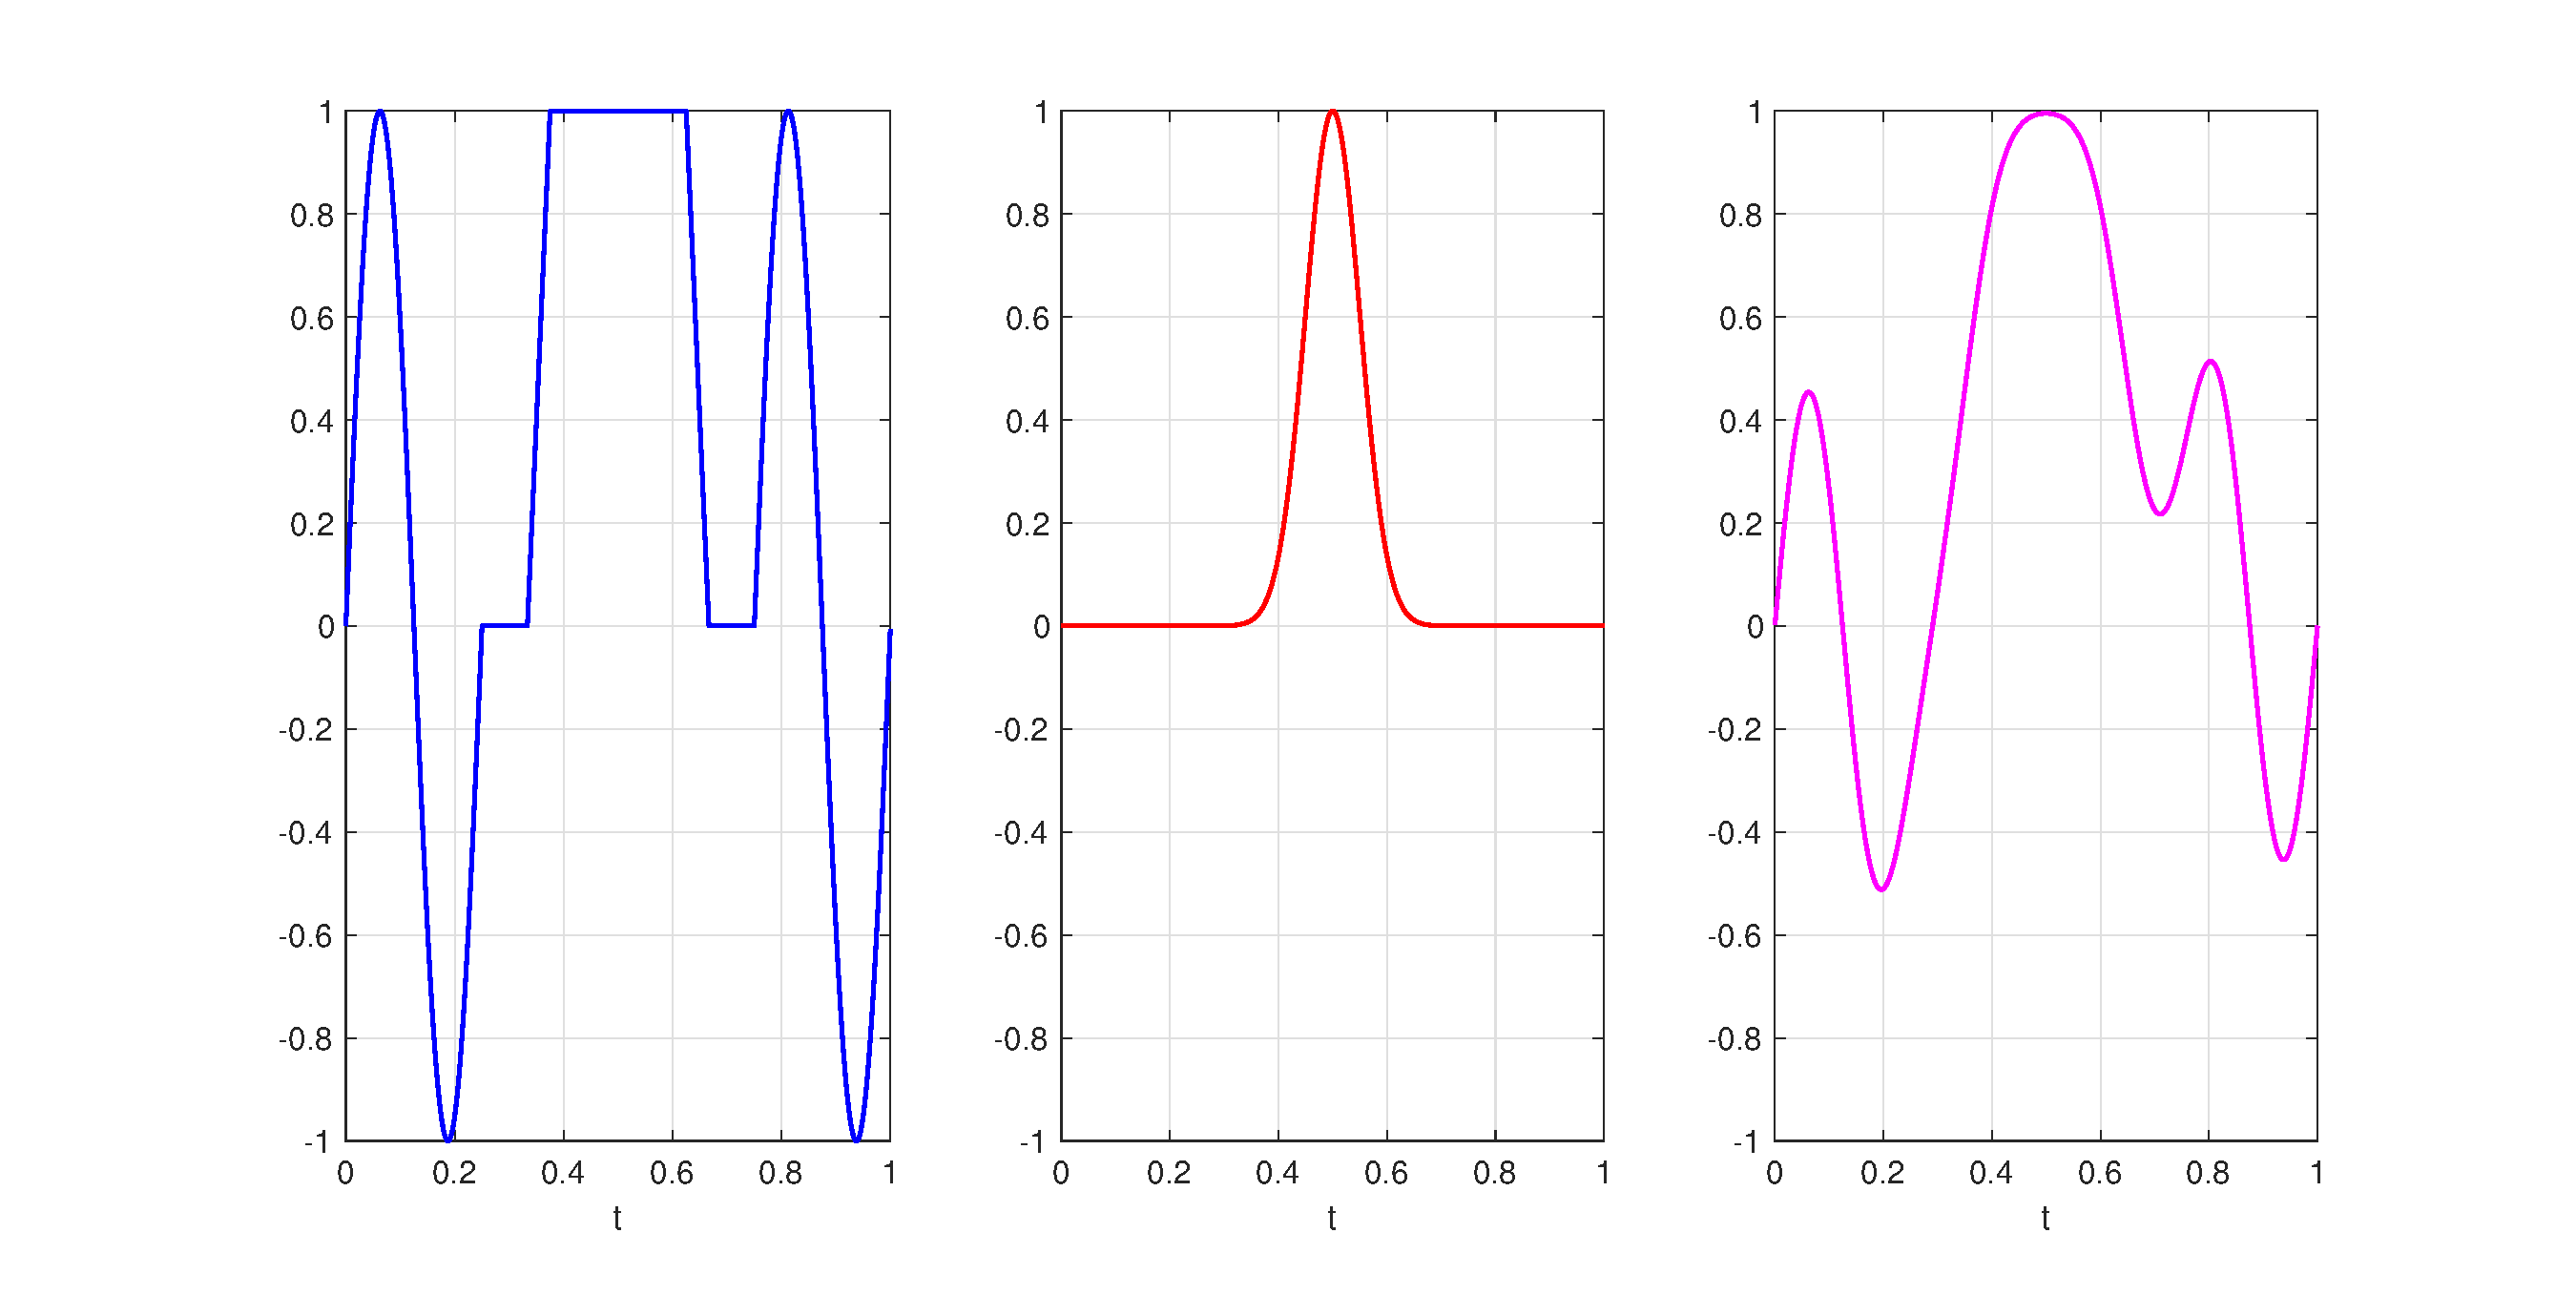
\includegraphics[scale=0.4]{Figures/FunctionKernelPlot.eps}}
\caption{Left: The graphs of the piecewise-smooth function $\fcon(t)$. Right: The Gaussian kernel $\kcon(t)$.}
\label{FunctionKernelPlot}
\end{figure}

\begin{figure}
	\centerline{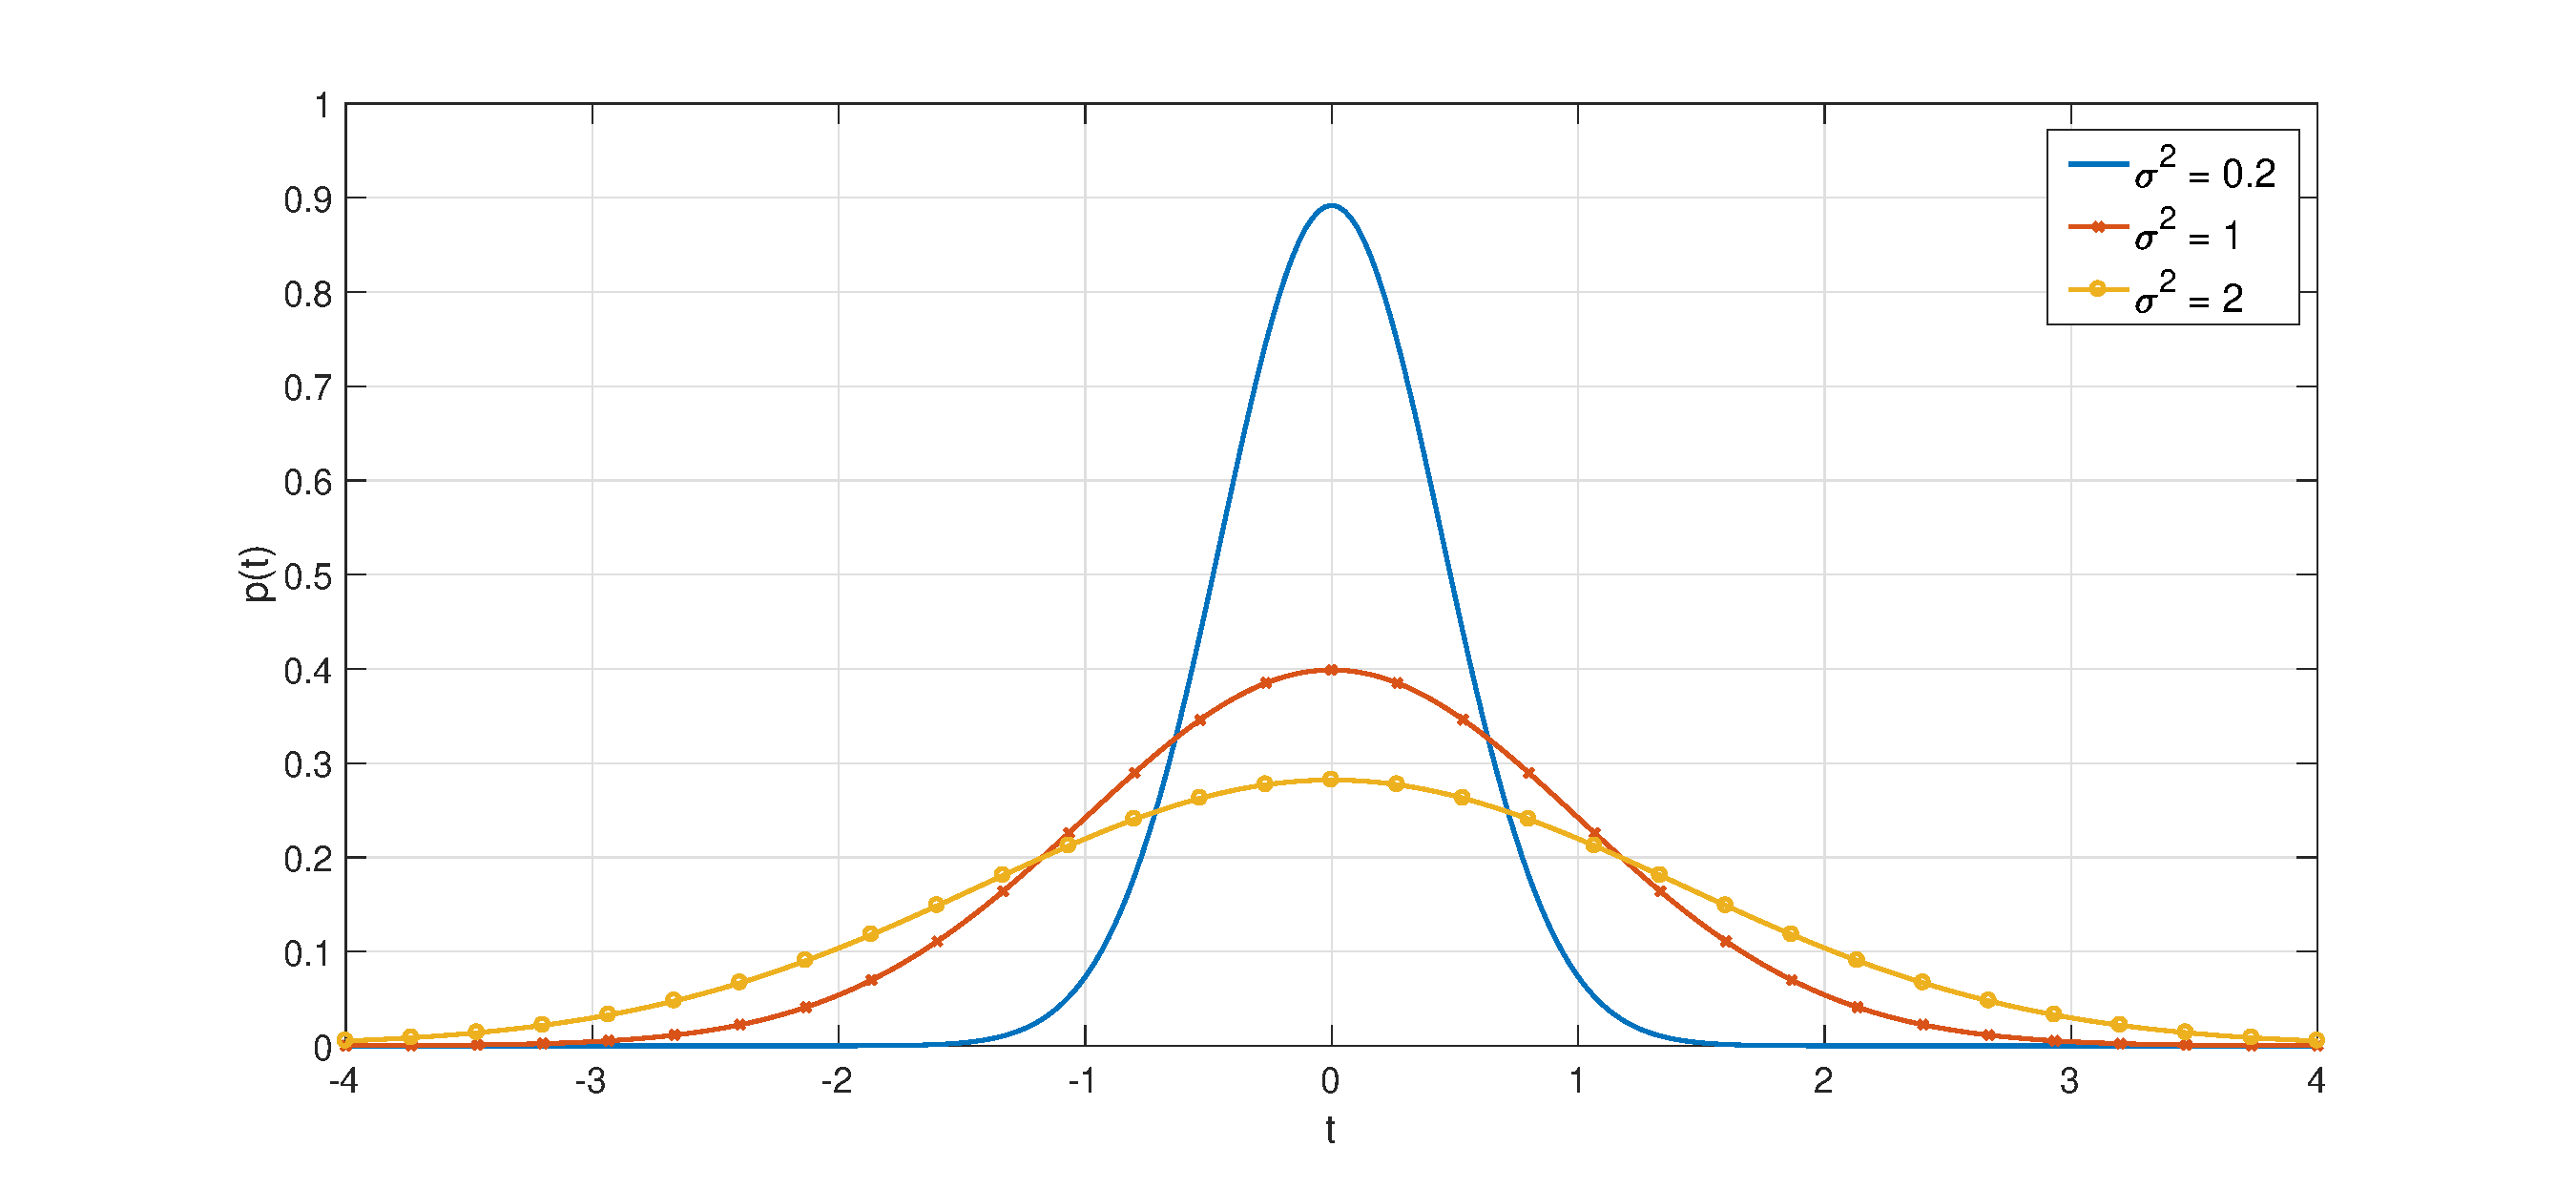
\includegraphics[scale=0.4]{Figures/GaussianDistributions.eps}}
\caption{Gaussian distributions for difference values of variance $\SD^2$, all centered at the origin ($\mu = 0$). As $\SD^2$ increases, the width of the distribution increases.}
\label{GaussianDistributions}
\end{figure}

To find a solution to the forward problem, which is the evaluation of $\gcon = \kcon * \fcon$, a quadrature method can be used to find a numerical approximation to the convolution integral. In the discrete setting, (1) can be stated as
\begin{equation}
\gdis = \kmat\fdis
\label{Eq_Dis}
\end{equation}
where $\fdis$ and $\gdis$ are the vector discretization of $\fcon$ and $\gcon$, respectively, and $\kmat$ is a matrix representing the discrete convolution of $\kcon$ with $\fcon$. For example, consider $\kcon(x,t)$ is a zero-centered Gaussian kernel and the domain of integration in \eqref{Eq_Con} is $[0,1]$. Given some $x_i \in [0,1]$, the continuous forward problem is to evaluate
\[g(x_i) = \int_0^1 \exp\left(\frac{-(x_i - t)^2}{2\SD^2}\right)\fcon(t) \: dt.\]
If a left Riemann sum is used with $t_j = (j-1)/n$ for $j \in \{1,2,\ldots,n\}$, representing an equispaced discretization of $[0,1]$ using $n$ points, then
\[g(x_i) \approx \sum_{j=1}^n \frac{1}{n}\exp\left(\frac{-(x_i - t_j)^2}{2\SD^2}\right)\fcon(t_j).\]
For approximations to $\gcon(x)$ at the same points that make up the equispaced discretization of $[0,1]$, i.e. at the points $x_i = (i-1)/n$ for $j \in \{1,2,\ldots,n\}$, then \eqref{Eq_Dis} is exactly the system that provides these approximations with $\fdis = [\fcon(t_1),\fcon(t_2),\ldots,\fcon(t_n)]$, $\gdis = [\gcon(x_1),\gcon(x_2),\ldots,\gcon(x_n)]$, and the elements of $\kmat$ being
\[K_{ij} = \frac{1}{n}\exp\left(\frac{-(i - j)^2}{2\SD^2}\right).\]
Note that taking the collocation and quadrature points as the same ensures that the matrix $\kmat$ is square. By changing the number of collocation points or the quadrature method can change $\kmat$ from square to rectangular. \par 
If the matrix $\kmat$ is nonsingular, then the solution to the inverse problem of \eqref{Eq_Dis} is $\fdis = \kmat^{-1}\gdis$. As with many linear systems, however, direct matrix inversion is discouraged and usually impractical since the matrix $\kmat$ becomes increasingly ill-conditioned as the size of the system grows [3]. Unfortunately, large systems are necessary to adequately approximate the continuous problem, and so other methods of solving for $\fdis$ must be considered. \par 
Another consequence of $\kmat$ being ill-conditioned relates to the accuracy of the vector $\gdis$. If $\gdis$ contains errors, as is often the case in practical applications, the errors are amplified during the multiplication $\kmat^{-1}\gdis$ since $\kmat$ is ill-conditioned and so the solution $\fdis$ will contain errors as well. For this consideration, the following system will be the assumed model throughout this report
\begin{equation}
\gnoise = \kmat\fdis + \noise
\end{equation}   
where $\noise$ is a vector that represents any errors in $\gdis$ (this is equivalent to the statement $\gnoise = \gdis + \noise$). For further simplicity, assume that $\noise \sim \mathcal{N}(\bm{0},\SD^2I)$, where $\bm{0}$ is the zero vector of length $n$ and $I$ is the $n \times n$ identity matrix. In other words, the error vector $\noise$ is an $n$-dimension Gaussian random variable with mean zero and variance $\SD^2$. \par 
Since direct matrix inversion is not practical, and at times not even possible since $\kmat$ can be non-invertible, a singular value decomposition (SVD) of $\kmat$ can be an alternative. Assuming $\kmat$ is a real $m \times n$ matrix of rank $r$, the SVD of $\kmat$ is 
\[\kmat = U\Sigma{V^\trans}\]
where the $m \times r$ matrix $U$ and the $r \times n$ matrix $V$ have orthogonal columns and $\Sigma$ is a $r \times r$ diagonal matrix. The diagonal elements of $\Sigma$ are the singular values of $\kmat$, denoted $\singular_i$ and satisfying $\singular_1 \geq \singular_2 \geq \ldots \geq \singular_r > 0$ where $r$ is the rank of $\kmat$. The columns of $U$ will be denoted $\LSV_i$ and $\RSV_i$ will denote the columns of $V$; these vectors are known as the left and right singular vectors of $\kmat$, respectively. A matrix of complex values has a SVD as well, the only difference being that the transpose is replaced with conjugate transpose. \par 
By using $\kmat^{-1} = V\Sigma^{-1}U^\trans$ when $\kmat$ is invertible, the product $\kmat^{-1}\gnoise$ is :
\[\kmat^{-1}\gnoise = \kmat^{-1}\left(\kmat\fdis + \noise\right) = \fdis + \kmat^{-1}\noise = \fdis + V\Sigma^{-1}{U^\trans}\noise = \fdis + \sum_{i = 1}^n \frac{{\LSV^\trans_i}\noise}{\singular_i}\RSV_i\]
For small $\singular_i$, the terms in the above sum are numerically unstable and must be modified. A common approach is to multiply the terms in the sum by \textit{filter functions} $\filt$ that depend upon $\singular_i$ and a \textit{regularization parameter} $\regparam$. By doing so, an approximate solution is obtained:
\begin{equation}
\fdis(\regparam) = \sum_{i = 1}^n \frac{\filt(\regparam,\singular_i){\LSV^\trans_i}\gnoise}{\singular_i}\RSV_i
\end{equation}

The most desired property of the filter functions is that $\filt(\singular_i)/\singular_i \approx 1$  for large values of $\singular_i$ and $\filt(\singular_i)/\singular_i \approx 0$ are small values of $\singular_i$. A brief overview of common filter functions will now be provided.

\subsection{Filter functions}
Perhaps the simplest filter function is
\[\filt(\regparam,\singular_i) = \begin{cases}
1, & \singular_i^2 > \regparam \\
0, & \singular_i^2 \leq \regparam
\end{cases}\]
Using this function in (3) gives the approximate solution
\[\fdis(\regparam) = \sum_{\singular_i^2 > \regparam} \frac{{\LSV^\trans_i}\gnoise}{\singular_i}\RSV_i\]
which actually corresponds to the solution obtained using a truncated singular value decomposition (TSVD) of the matrix $\kmat$ [3]. \par 
A less simple filter function is
\begin{equation}
\filt(\regparam,\singular_i)  = \frac{\singular_i^2}{\singular_i^2 + \regparam}
\end{equation}
which is known as the Tikhonov filter function. For large values of $\regparam$, the above fraction is close to zero and for small values of $\regparam$, the fraction is near to unity. The use of the Tikhonov filter function to generate an approximate solution is known as \textit{Tikhonov regularization}; the obtained solution is 
\[\fdis(\regparam) = \sum_{i = 1}^n \frac{\singular_i^2}{\singular_i^2 + \regparam}\frac{{\LSV^\trans_i}\gnoise}{\singular_i}\RSV_i = \sum_{i = 1}^n \frac{\singular_i{\LSV^\trans_i}\gnoise}{\singular_i^2 + \regparam}\RSV_i \]
An alternative representation of the above Tikhonov solution is
\begin{equation}
\fdis(\regparam) = \arg\min_{\fdis \in \mathbb{R}^n} \|\kmat\fdis - \gnoise\|^2 + \regparam\|\fdis\|^2
\end{equation}
The term $\|\fdis\|^2$ is commonly called the penalty function [3], and is actually a specific case of the more general penalty function $\|L\fdis\|^2$ where $L$ is a linear operator (here $L = I$, the $n \times n$ identity matrix).

The kernel $k$ and function $f$ considered in the introduction will be retained for the numerical examples included in this report. 

\section{Analytical tools}

\subsection{Discrete convolution}
As described in the Introduction, the operation of convolution arises in various settings pertaining to inverse problems. Discrete convolution will first be described  in a general setting, followed by specific instances and connections to the numerical experiments conducted in this report. \par 



\subsection{The Fourier transform}

\section{Experiment design}
 
For the numerical experiments, three test functions are considered. While these functions vary in the extent of smoothness, all three functions are selected to be 1-periodic and the interval selected is [0,1], though this interval can be mapped to any other interval using a linear transformation. In general, the transformation from $[a,b]$ to $[c,d]$ such that $a \mapsto c$ and $b \mapsto d$ has a point-slope representation
\[y - c = \left(\frac{d-c}{b-a}\right)(x - a)\]
where $y \in [c,d]$ is the image of $x \in [a,b]$. \par 
The first test function is $\fcon(x) = \cos(4\pi{t})\sin(6\pi{t})$, which is infinitely differentiable on all of $\mathbb{R}$. The second test function \eqref{Eq_TF2} is piecewise-smooth. The third and final test function is
\begin{equation}
\fcon(x) = \cos(8\pi{t})\exp(\sin(10\pi{t})-1)
\label{Eq_TF3}
\end{equation}
which is also infinitely differentiable on $\mathbb{R}$; the third function was selected to be more interesting than the first test function. Graphs of all three test functions are found in Figure \ref{TestFunctions}.  \par 

\begin{figure}
	\centerline{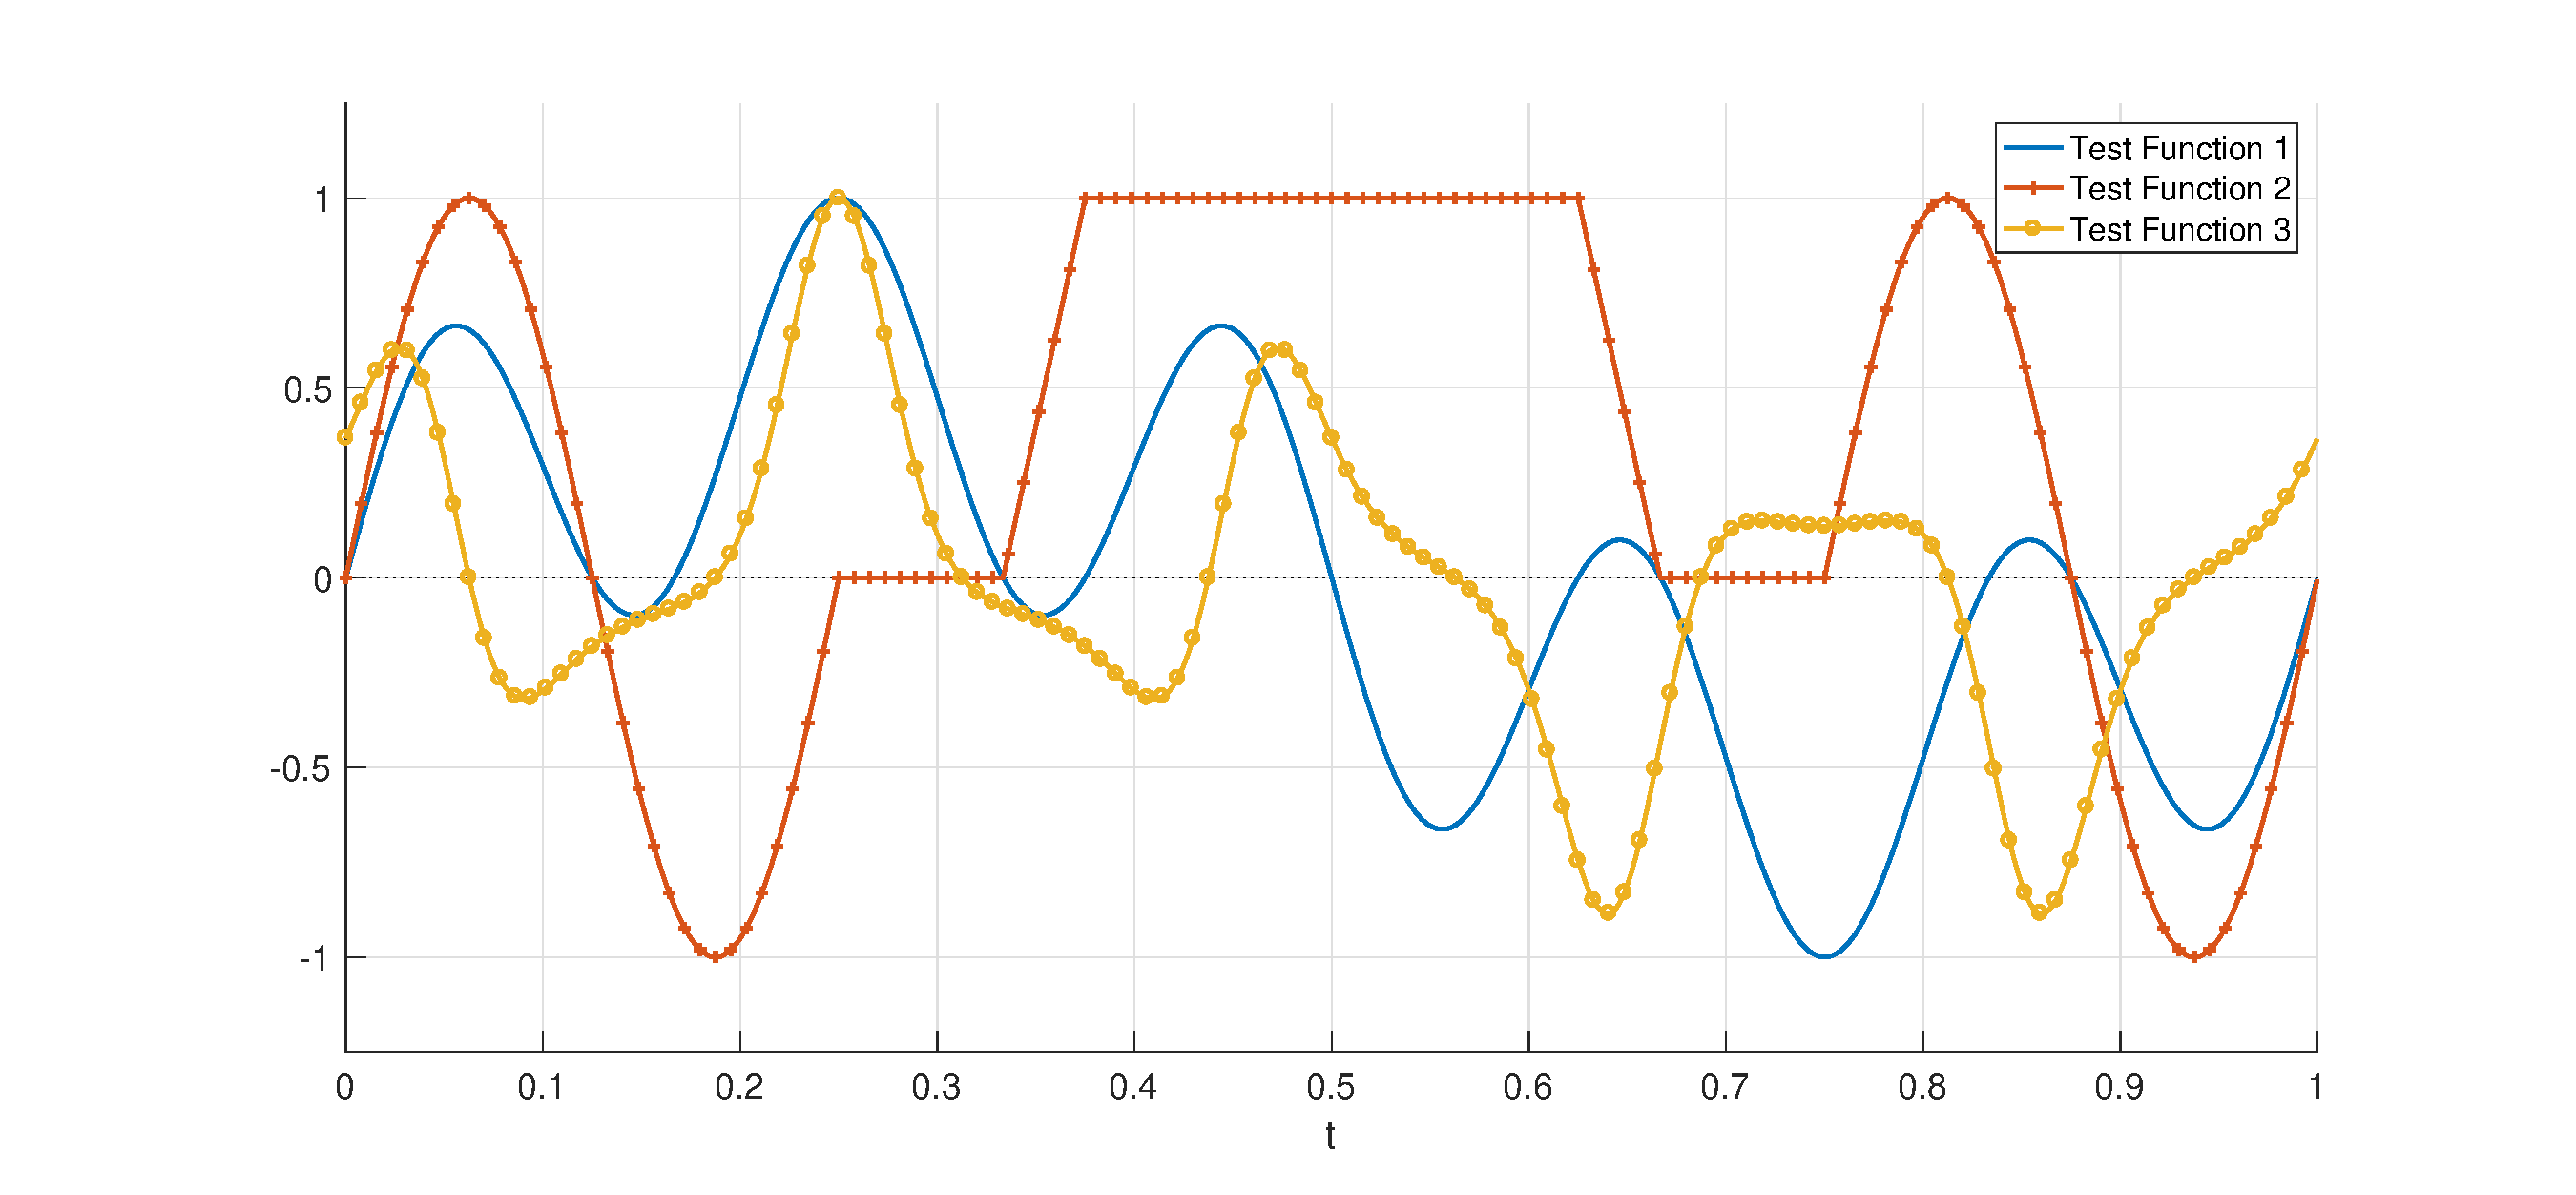
\includegraphics[scale = 0.45]{Figures/TestFunctions1D.eps}}
\caption{The three test functions considered in the numerical experiments. Note that the second test function is only piecewise-smooth, while the first and second functions are smooth. All three functions are 1-periodic.}
\label{TestFunctions}
\end{figure}

The interval $[0,1]$ is discretized as equispaced points $0, 1/N, 2/N, \ldots, (N-1)/N$ for $N = 4096$. In other words, the interval is discretized as the vector $\tdis = [t_1,t_2,\ldots,t_N]$ with $t_i = (i-1)/N$. The selected test function $\fcon$ is then sampled at these points so that the discrete version $\fdis = [\fcon_1,\fcon_2,\ldots,\fcon_N]$ has elements $\fcon_i = \fcon(t_i)$. For the discrete version of $\kcon$ to be used in the convolution with $\fdis$, the periodic extension of $\kcon$ is sampled in the same way that was used to construct $\fdis$. However, it is important to remember that unextended $\kcon(t)$ was assumed to be centered at the origin and compactly supported on the interval $[-1/2,1/2]$. As such, a plot of $\kdis$ will not resemble the traditional graph of a Gaussian bump but instead be a depiction of a trough between bumps in the periodic extension of $\kcon$; see Figure \ref{RegAndTroughGaussian}. In the experiments, the radii of the Gaussian kernels are chosen to be 50 and 100.  \par 

\begin{figure}
	\centerline{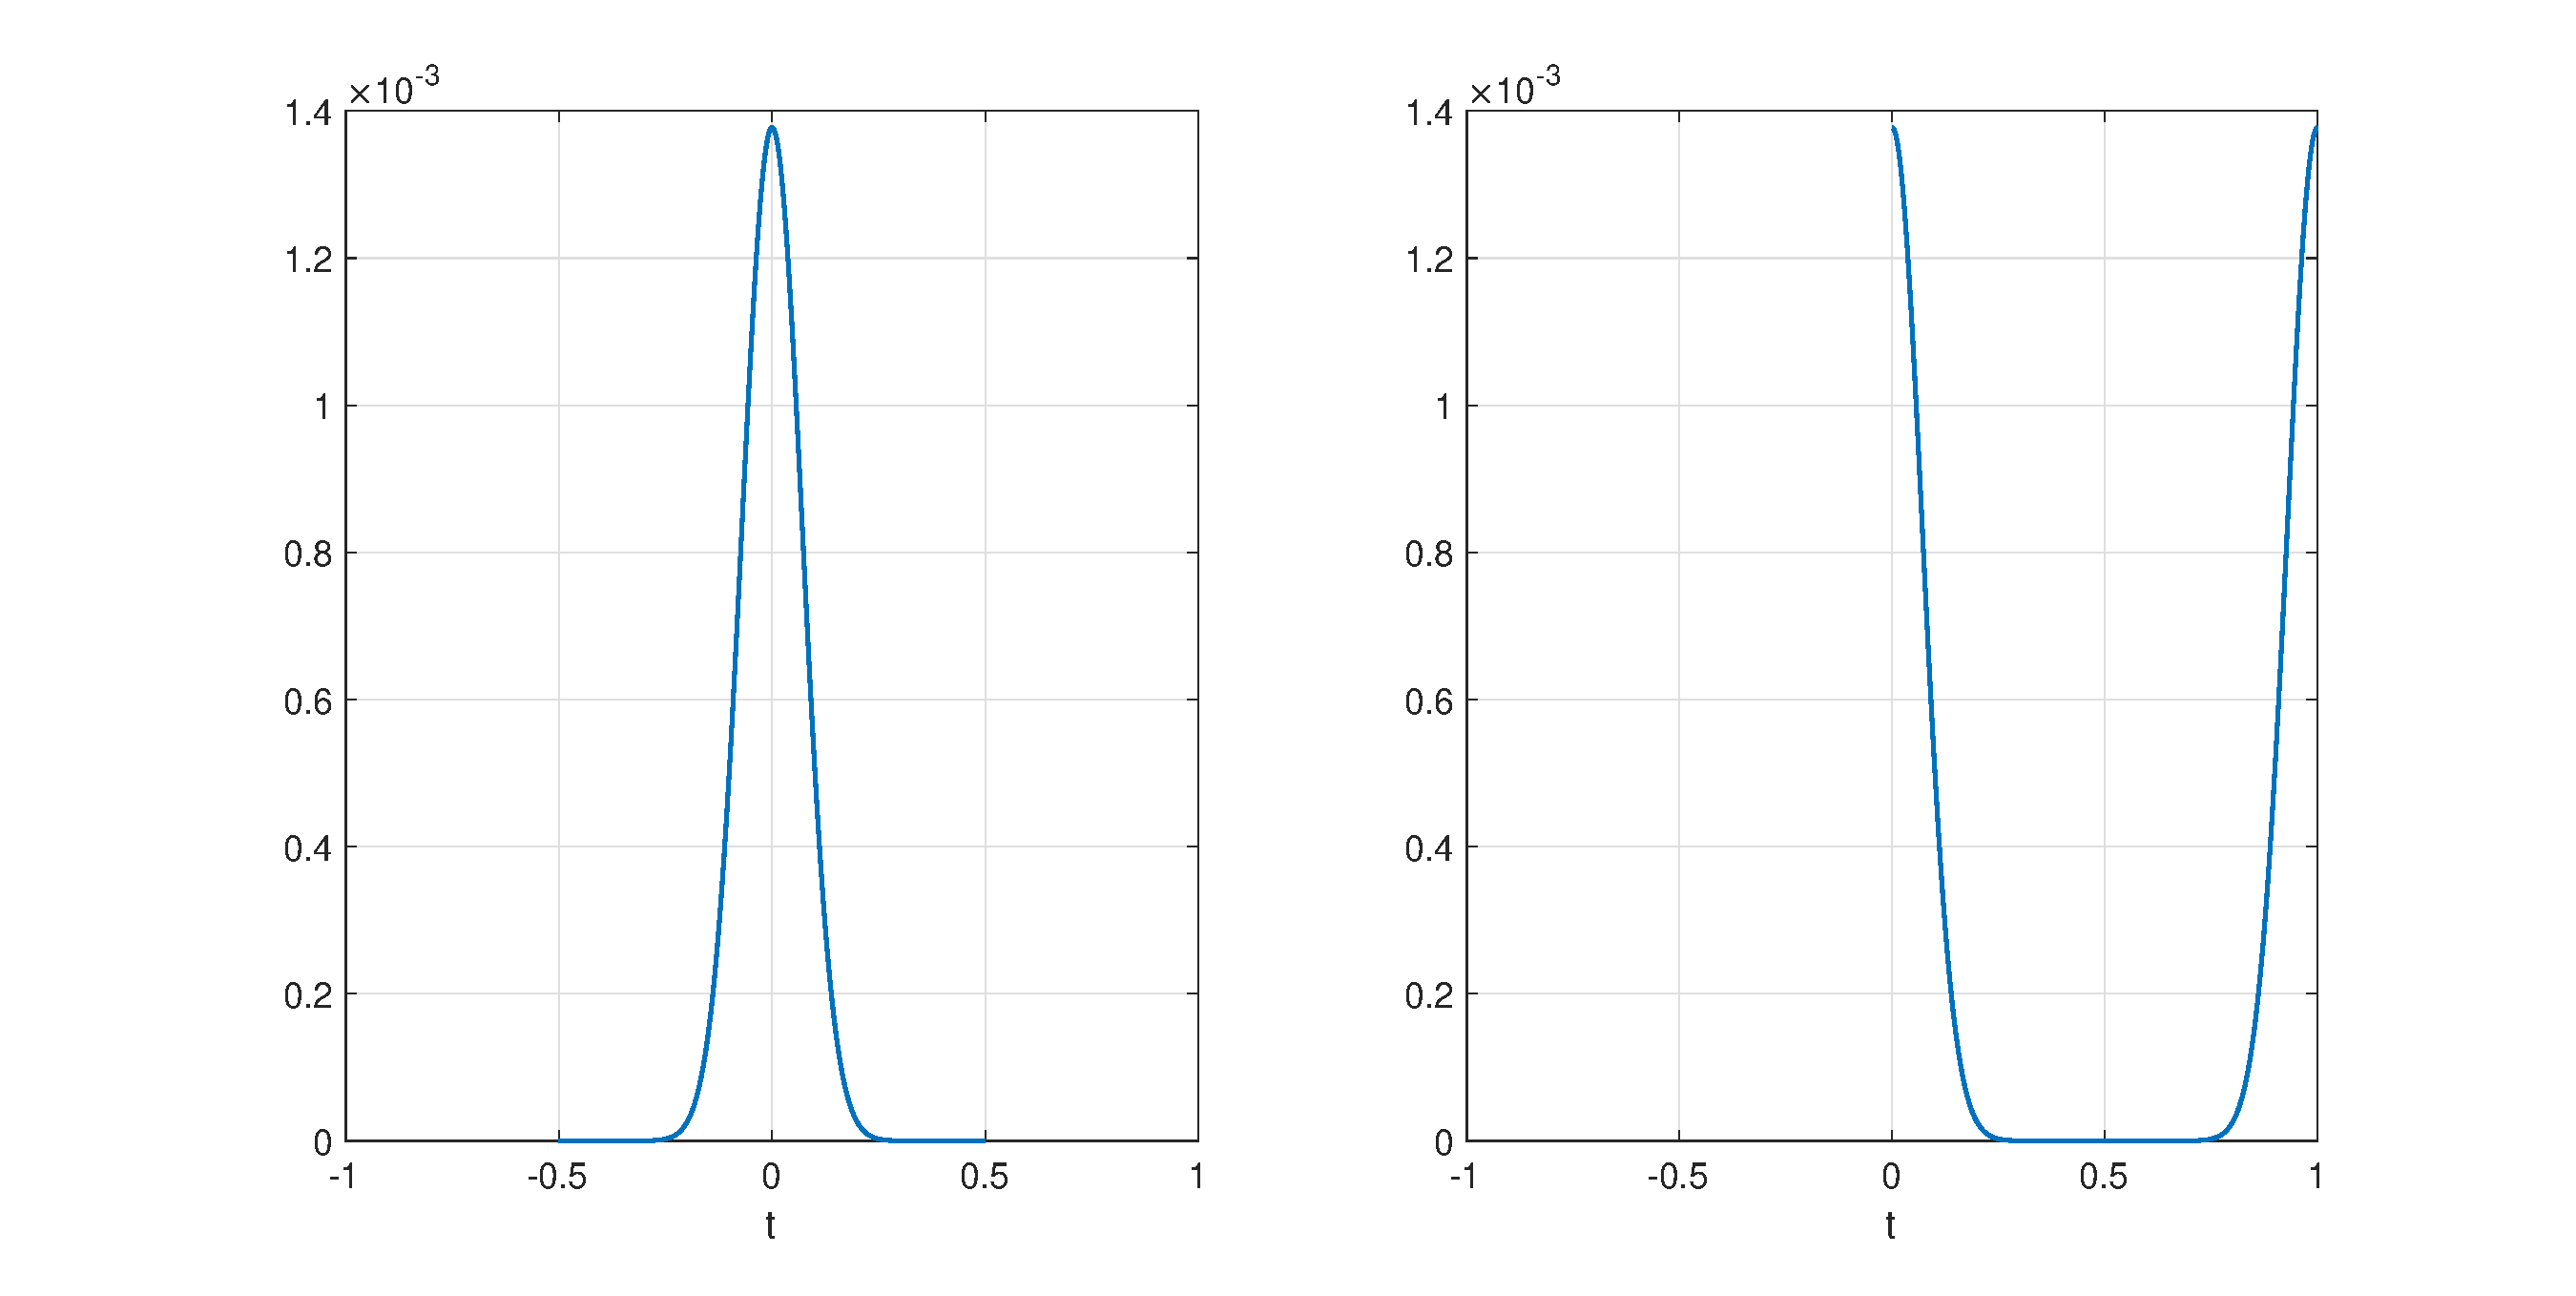
\includegraphics[scale = 0.45]{Figures/RegAndTroughGaussian.eps}}
\caption{Plots of different discretizations of the kernel $\kcon(t)$. The discretization on the left reflects the compact support of $\kcon$ on the interval $[-1/2,1/2]$. The discretization on the right represents the periodic extension of $\kcon$ on the interval $[0,1]$.}
\label{RegAndTroughGaussian}
\end{figure}

With the discretizations $\fdis$ and $\kdis$ determined, the discretization $\gdis$ of $\gcon(t)$ can be evaluation using either a circular convolution or a linear convolution with appropriate vector padding (see subsection on convolution, which needs to be added). Ultimately the vectors $\fdis$, $\kdis$, and $\gdis$ are vector discretizations of $\fcon$, $\kcon$, and $\gcon$, respectively.

Overall, two selections for the width of the Gaussian kernel, two selections for SNR value, and three test functions lead to a total of 12 experimental configurations. For each configuration, 20 noise realizations were generated and tested. The full resolution problem was constructed using $N = 4096$ points. The downsamped resolutions were selected as $n \in \{16,32,\ldots,2048\}$ for a total of nine resolutions (eight values of $n$).

\subsection{Construction of noise}

Though the definition of SNR varies, the definition chosen for this investigation is
\begin{equation}
\label{Eq_SNR}
\text{SNR} = 10\log_{10}\left(\frac{P_{\text{signal}}}{P_{\text{noise}}}\right)
\end{equation}
where $P$ denotes average power. In the discrete setting, the average power of a signal $\mathbf{f}$ of length $N$ is defined as $\|\mathbf{f}\|^2/N$. Using this definition, $P_{\text{signal}} = \|\gdis\|^2/N$ and $P_{\text{noise}} = \|\noise\|^2/N$ and so the quotient in the logarithm is $\|\gdis\|^2/\|\noise\|^2$. The quotient can also be expressed as $(\|\gdis\|/\|\gnoise - \gdis\|)^2$, which is the square of the multiplicative inverse of the relative error of $\gnoise$. \par 
In MATLAB, the noise vector $\noise$ can be constructed by first taking an $N$-vector $\mathbf{e}$ drawn from the multivariate standard normal distribution and multiplying the vector by a constant $\SD$. Doing so ensures that $\noise$ has variance $\SD^2$ because $\Var(\noise) = \Var(\SD\:\mathbf{e}) = \SD^2\:\Var(\mathbf{e})$ and $\mathbf{e}$ has unit variance. Thus it is useful to rearrange the equation defining SNR into an equation that provides a way of finding the necessary variance for a given SNR value. The rearrangement is shown below, with $\|\noise\|^2$ replaced by $\E(\|\noise\|^2)$.
\[\E(\|\noise\|^2) = \frac{\|\gdis\|^2}{10^{(\text{SNR}/10)}}\]
Using the properties of expected value and the fact that $\E(\|\noise\|^2) = \E(\|\SD\:\mathbf{e}\|^2)$, the term on the left hand side of the equation can be changed as
\[\E(\|\noise\|^2) = \E(\|\SD\:\mathbf{e}\|^2) = \SD^2 \sum_{i=1}^N \E(\mathbf{e}_i^2) = \SD^2 \sum_{i=1}^N \left(\E(\mathbf{e}_i)^2 + \Var(\mathbf{e}_i)\right) = \SD^2 \sum_{i=1}^N \left(0^2 + 1\right) = \SD^2\:N.\]
Utilizing this change, the following equation for variance is obtained.
\begin{equation}
\label{Eq_Var}
\SD^2 = \frac{\|\gdis\|^2}{N \cdot 10^{(\text{SNR}/10)}} 
\end{equation}
This equation is used for the numerical construction of the noise vectors. SNR values of 5 and 25 are used to generate the white noise added to $\gdis$, and one such data realization is shown in Figure \ref{NoisePlot1D_F2_S05_W200}. \par  

\begin{figure}
	\centerline{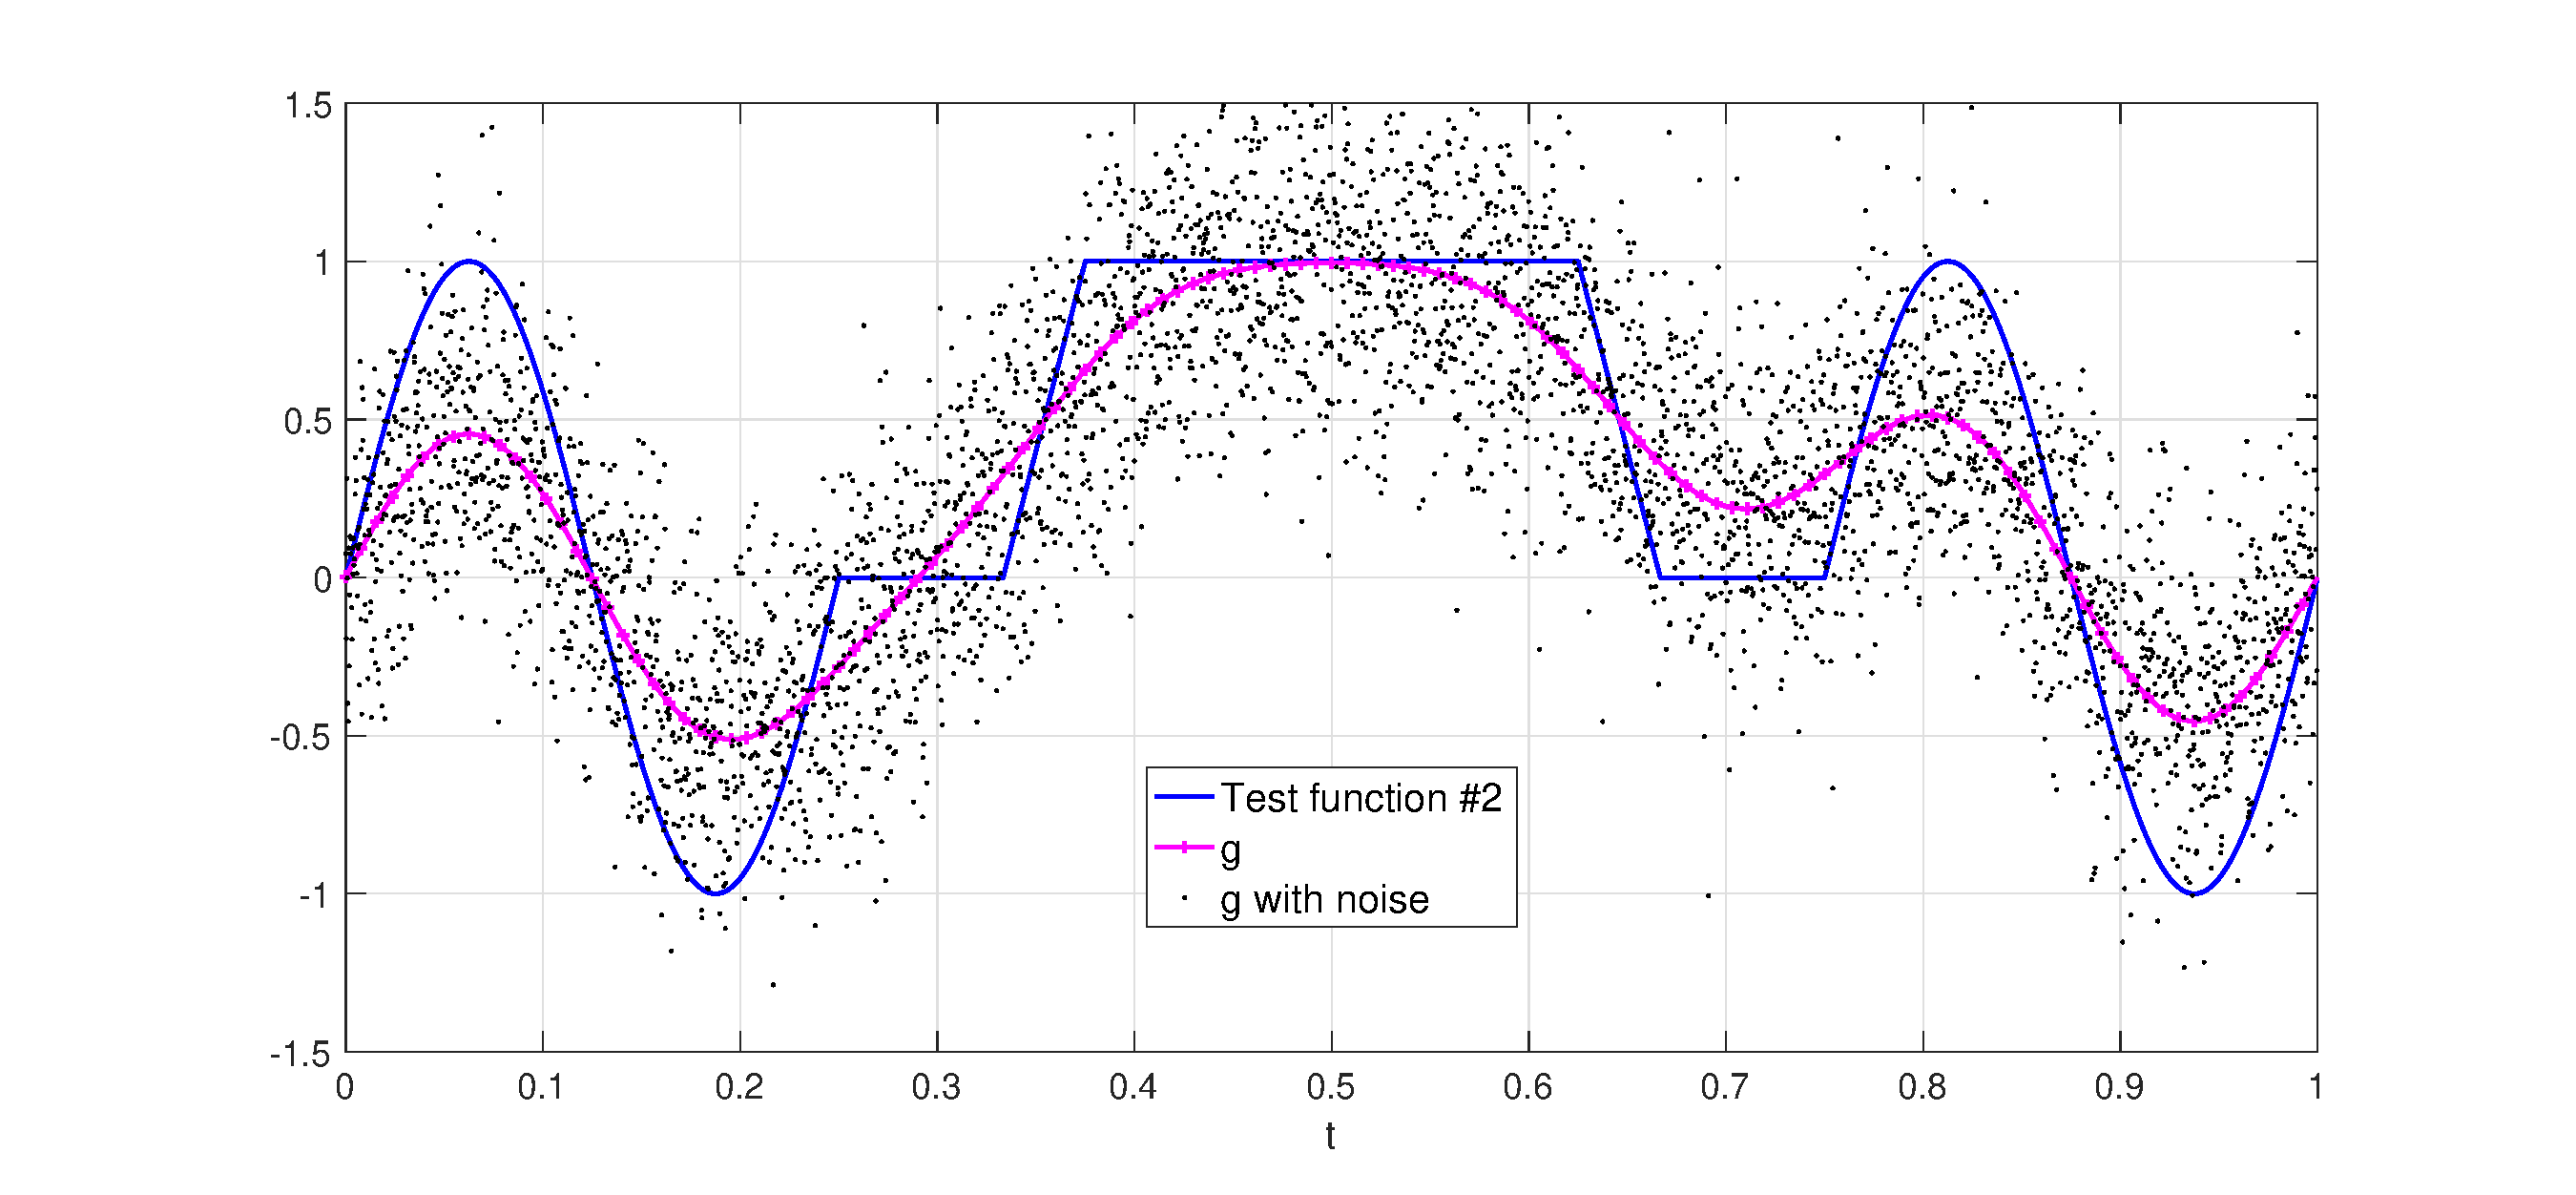
\includegraphics[scale = 0.45]{Figures/NoisePlot1D_F2_S05_W200.eps}}
\caption{The plot shows one data realization of $\gdis$ with noise, where the original function $f$ was the second test function. The SNR value is 5 and the radius of the Gaussian PSF is 100.}
\label{NoisePlot1D_F2_S05_W200}
\end{figure}
 
For an accurate evaluation of the numerical experiments and their results, multiple realizations of noise are used. A primary advantage of multiple noise realizations is that the sample variance of noise vectors approaches the desired variance as the number of realizations increases. More rigorously, the mean of the sample variances of the noise vectors converges almost surely to the expected value of the sample variance, which is the desired variance $\SD^2$; this is a direct consequence of the (strong) law of large numbers and the fact that the noise vectors are independent and identically distributed with standard normal distribution. Figure \ref{LLN_Plot} depicts the law of large numbers as applied to noise realizations.  \par 

\begin{figure}
\centerline{\includegraphics[scale=0.45]{Figures/LLN_Plot.eps}}
\caption{The three plots correspond to the noise vectors generated using each of the three test functions (the right hand side of equation \eqref{Eq_Var} depends upon $\gdis$, which depends upon the test function $\fdis$ and the width of the Gaussian kernel). Equation \eqref{Eq_Var} also depends upon SNR; a SNR of 5 and Gaussian kernel width of 50 was used in all three cases. The horizontal axis represents the number of noise realization and the vertical axis represents sample variance. All three plots show that as the number of realizations increases, the mean of the sample variances approaches the desired sample variance (the left hand side of equation \eqref{Eq_Var} and the red line in the plots).}
\label{LLN_Plot}
\end{figure}

Another numerical consideration regarding noise is how the sample variance changes across downsampling resolutions. To formalize the concept of downsampling in the context of this report, consider $\mathbf{z} = [z_1,z_2,\ldots,z_n]$. Then a vector $\mathbf{y}$ is called a downsampling of $\mathbf{z}$ if $\mathbf{y} = [z_{n_1},z_{n_2},\ldots,z_{n_m}]$, where $m \leq n$ and $n_j:\{1,2,\ldots,m\}\rightarrow\{1,2,\ldots,n\}$ is a strictly increasing function. This definition is analogous to the definition of a subsequence except with a finite number of terms. \par  
Theoretically, the variance of the noise vector does not change when a vector is downsampled because of the properties of variance. For any $m\times n$ matrix $M$ and $n$-vector $\noise \sim \mathcal{N}(\bm{0},\SD^2I)$
\begin{equation}
\Var(M\noise) = M\Var(\noise)M^{\trans} = \SD^2MIM^{\trans} = \SD^2MM^{\trans}
\label{Eq_VarProp}
\end{equation}
where $MM^\trans$ is an $m \times m$ matrix. Certainly for arbitrary $M$, $MM^\trans$ can differ from an $m \times m$ identity matrix, which would mean that the new noise vector $M\noise$ no longer represents white noise. However, given an $n$-vector $\noise \sim \mathcal{N}(\bm{0},\SD^2I)$ and the goal of obtaining a downsampled version of $\noise$, a matrix $E$ can be found such that $E\noise$ is the downsampled vector. Since DFT's are utilized in the regularization process, a downsampled vector whose components are still equidistant from adjacent components is desirable. Since the finest sampling $\tdis$ of the interval $[0,1]$ has $N = 4096 = 2^{12}$ points, a natural downsampling with this property would be to select every other component of $\tdis$. The resulting downsampled vector would then have length $N/2 = 2048 = 2^{11}$. The matrix $E$ that accomplishes this downsampling is the $N/2 \times N$ matrix defined as
\begin{equation}
E = [\mathbf{e}_1 \: \mathbf{0} \: \mathbf{e}_2 \: \mathbf{0} \: \mathbf{e}_3 \: \mathbf{0} \ldots \mathbf{e}_N]
\label{Eq_E}
\end{equation}
where $\mathbf{0}$ is the $N/2$-vector of all zeros and $\mathbf{e}_j$ is the $N/2$-vector of all zeros except for 1 as the $j\text{th}$ component, $1 \leq j \leq N/2$. In an effort to clarify this downsampling process, let $\tdis^{n}$ denote the $n$-point downsampling of $\tdis$. Then with this new notation, $\tdis^{2046} = E\tdis$. \par 
As a smaller example, consider the vector
\[\tdis = \begin{bmatrix}
0 & \dfrac{1}{8} & \dfrac{1}{4} & \dfrac{3}{8} & \dfrac{1}{2} & \dfrac{5}{8} & \dfrac{3}{4} & \dfrac{7}{8}
\end{bmatrix}^{\trans}\]
which is an equispaced 8-point discretization of $[0,1]$. The $4 \times 8$ matrix $E$ used to obtain downsampling $\tdis^{4}$ is
\[E = \begin{bmatrix}
1 & 0 & 0 & 0 & 0 & 0 & 0 & 0 \\
0 & 0 & 1 & 0 & 0 & 0 & 0 & 0 \\
0 & 0 & 0 & 0 & 1 & 0 & 0 & 0 \\
0 & 0 & 0 & 0 & 0 & 0 & 1 & 0 \\
\end{bmatrix}.\]
Then $\tdis^4$ obtained by the product $E\tdis$ has equispaced components as desired:
\[\tdis^4 = E\tdis = \begin{bmatrix}
0 & \dfrac{1}{4} & \dfrac{1}{2} & \dfrac{3}{4}
\end{bmatrix}^{\trans}.\]
\indent Another property of the $N/2 \times N$ matrix $E$ defined in \eqref{Eq_E} is that $EE^{\trans} = I$, where $I$ is the $N/2 \times N/2$ identity matrix.  This is a direct consequence of $\mathbf{e}_j^\trans\mathbf{e}_j = 1$ for all $j$ with $1 \leq j \leq N/2$. Using the property in \eqref{Eq_VarProp}, the variance of the  noise vector $\noise^{N/2}$ downsampled from $\noise$ is then
\[\Var(\noise^{N/2}) = \Var(E\noise) = E\Var(\noise)E^{\trans} = \SD^2EE^{\trans} = \SD^2I\]
where $I$ is the $N/2 \times N/2$ identity matrix. Therefore, downsampling white noise vectors in this way produces white noise vectors of half length, theoretically preserving variance across downsamples. As a final remark, the process of downsampling described here can be used to obtain downsampled vectors of length $N/(2^2), N/(2^3), \ldots, N/N$, though the final resolution in this report has been chosen as $N/(2^8) = 16$. \par 
While in theory the variance of downsampled vectors is the same across resolutions, numerically 

\section{Parameter estimation methods}

\subsection{Unbiased Predictive Risk Estimator}
The Unbiased Predictive Risk Estimator (UPRE) method is derived by considering the following quantity
\[\PE := \kmat(\freg - \fdis)\]
This quantity $\PE$ is known as the \textit{predictive error}, and is an alternative to solution error defined as $\freg - \fdis$. Given the above definition, the mean squared norm of the predictive error is
\[\frac{1}{n}\|\PE\|^2 = \frac{1}{n}\|\kmat(\freg - \fdis)\|^2\]
which is called the predictive risk.  As a first step in deriving the UPRE method, assume that the noise $\noise$ is a random vector, instead of a realization of a random vector. Direct consequences of this assumption are that $\gdis$ and $\freg$ are random vectors and the predictive risk $(1/n)\|\PE\|^2$ is a random variable. \par 
Next, an $n \times n$ matrix $\A$ is defined as $\A = \kmat\R$ where $\R$ is a regularization matrix. The notation $\A$ is chosen to indicate that the matrix depends upon the regularization parameter contained in $\R$. Using the influence matrix with $\freg = \R\gnoise$, the predictive error can be rewritten:
\begin{align*}
\PE &= \kmat\freg - \kmat\fdis \\
&= \A\gnoise - \kmat\fdis \\
&= \A(\kmat\fdis + \noise) - \kmat\fdis \\
&= (\A - I)\kmat\fdis + \A\noise
\end{align*}
By the assumption that $\noise$ is a discrete white noise vector, the Trace Lemma can be utilized to obtain an expression for the expected value of predictive risk.
 
\begin{TL}
Let $f \in \mathcal{H}$, where $\mathcal{H}$ is a deterministic, real Hilbert space, let $\noise$ be a discrete noise vector with $\noise \sim \mathcal{N}(0,\SD^2)$, and let $B: \mathbb{R}^n \rightarrow \mathcal{H}$ be a bounded linear operator. Then
\[\E(\|f + B\noise\|_{\mathcal{H}}^2) = \|f\|_{\mathcal{H}}^2 + \SD^2\trace({B^*}B)\]
where $B^*$ denotes the adjoint of $B$.
\end{TL}
\begin{proof}
By the linearity of inner products and the expected value operator,
\[\E(\|f + B\noise\|_{\mathcal{H}}^2) = \E(\langle f + B\noise, f + B\noise\rangle_{\mathcal{H}}) = \E(\|f\|_{\mathcal{H}}^2) + 2\E(\langle f, B\noise\rangle_{\mathcal{H}}) + \E(\langle B\noise, B\noise\rangle_{\mathcal{H}}).\]
The term $\E(\|f\|_{\mathcal{H}}^2)$ reduces to $\|f\|_{\mathcal{H}}^2$ because $f$ is an element of a deterministic Hilbert space. Next, the inner products can be rewritten using the adjoint of $B$:
\begin{align*}
\E(\|f + B\noise\|_{\mathcal{H}}^2) &= \|f\|_{\mathcal{H}}^2 + 2\E(\langle f, B\noise\rangle_{\mathcal{H}}) + \E(\langle B\noise, B\noise\rangle_{\mathcal{H}}) \\
&= \|f\|_{\mathcal{H}}^2 + 2\E(({B^*}f)^\trans\noise) + \E({\noise^\trans}{B^*}B\noise) \\
&= \|f\|_{\mathcal{H}}^2 + 2\sum_{i=1}^n ({B^*}f)_i \E(\noise_i) + \sum_{i=1}^n\sum_{j=1}^n ({B^*}B)_{ij} \E({\noise_i}{\noise_j})
\end{align*}
Since $\noise \sim \mathcal{N}(0,\SD^2)$, the expected values of $\noise_i$ and ${\noise_i}{\noise_j}$ are zero and $\SD^2\delta_{ij}$, respectively. Therefore the second term above is zero and the third term is a summation expression for $\SD^2\trace({B^*}B)$.
\end{proof}

\noindent Applying the Trace Lemma to the expression for predictive risk yields
\[\E\left(\frac{1}{n}\|\PE\|^2\right) = \frac{1}{n}\E\left(\|(\A-I)\kmat\fdis + \A\noise\|^2\right) = \frac{1}{n}\|(\A-I)\kmat\fdis\|^2 + \frac{\SD^2}{n}\trace({\A^\trans}\A).\]
If Tikhonov regularization is used, then the influence matrix $\A$ is $\kmat(\kmat^\trans\kmat + \regparam{I})^{-1}\kmat^\trans$. The matrix $(\kmat^\trans\kmat + \regparam{I})^{-1}$ is symmetric as a result of $\kmat^\trans\kmat$ and $\regparam{I}$ being individually symmetric, and thus the corresponding influence matrix $\A$ is symmetric.  With a symmetric matrix $\A$, the expected value of predictive risk is simplified to
\begin{equation}
\label{Eq_PR}
\E\left(\frac{1}{n}\|\PE\|^2\right) = \frac{1}{n}\|(\A-I)\kmat\fdis\|^2 + \frac{\SD^2}{n}\trace(\A^2).
\end{equation}
\indent The last step in the derivation of the UPRE method is to introduce the \textit{regularized residual}, which is defined as $\regres = \kmat\freg - \gnoise$. The regularized residual is important because it is also used in the derivation of the generalized cross validation and discrepancy principle methods. Using the influence matrix $\A$, the expression for $\regres$ can also be written as
\[\regres = (\A-I)\gnoise = (\A-I)(\kmat\fdis + \noise) = (\A-I)\kmat\fdis + (\A-I)\noise.\]
By the Trace Lemma and the expression for $\regres$, the expected value of $(1/n)\|\regres\|^2$ is
\[\E\left(\frac{1}{n}\|\regres\|^2\right) = \frac{1}{n}\|(\A-I)\kmat\fdis\|^2 + \frac{\SD^2}{n}\trace({(\A-I)^\trans}(\A-I))\]
For symmetric $\A$, the term $(\A-I)^\trans(\A-I)$ becomes $(\A-I)^2 = \A^2 - 2\A + I$ and so by the linearity of the trace operator,
\begin{equation}
\label{Eq_RR}
\E\left(\frac{1}{n}\|\regres\|^2\right) = \frac{1}{n}\|(\A-I)\kmat\fdis\|^2 + \frac{\SD^2}{n}\trace(\A^2) - \frac{2\SD^2}{n}\trace(\A) + \SD^2.
\end{equation} 
By comparing \eqref{Eq_PR} and \eqref{Eq_RR}, the equation for the expected value of $(1/n)\|\PE\|^2$ can be expressed as
\[\E\left(\frac{1}{n}\|\PE\|^2\right) = \E\left(\frac{1}{n}\|\regres\|^2\right) + \frac{2\SD^2}{n}\trace(\A) - \SD^2.\]
The UPRE is defined to be
\begin{equation}
\label{Eq_UPRE}
\U(\regparam) = \frac{1}{n}\|\regres\|^2 + \frac{2\SD^2}{n}\trace(\A) - \SD^2
\end{equation}
and the UPRE method is to pick $\regparam$ as the minimizer of $\U(\regparam)$. 

\subsection{Generalized Cross Validation}
The UPRE method requires knowledge of the variance $\SD^2$ of the noise vector $\noise$. In contrast, the generalized cross validation (GCV) method does not require knowledge of $\SD^2$. The GCV functional is
\begin{equation}
\label{Eq_GCV}
\GCV(\regparam) = \frac{\frac{1}{n}\|\regres\|^2}{\left[\frac{1}{n}\trace(I-\A)\right]^2},
\end{equation}
where $\regres$ is the regularized residual defined in the derivation of the UPRE method. Similarities between the GCV and UPRE methods are that both functionals are estimators of the predictive risk, and the regularization parameter $\regparam$ is chosen as the minimizers of these functionals.

\subsection{Discrepancy Principle}
As a start to a stochastic derivation of the discrepancy principle method (for a deterministic derivation, see [3]), consider the case where $\freg \approx \fdis$. In this case, 
\[\regres = \kmat\freg - \gnoise \approx \kmat\fdis - \gnoise = \noise.\]
with a direct consequence being that $\E((1/n)\|\regres\|^2) \approx \E((1/n)\|\noise\|^2) =\SD^2$. Thus the discrepancy principle is to choose $\regparam$ such that $(1/n)\|\regres\|^2 = \SD^2$.
Implementation of this method requires finding a solution of $\D(\regparam) = 0$, where $\D(\regparam)$ is defined to be
\begin{equation}
\label{Eq_DP}
\D(\regparam) = \frac{1}{n}\|\regres\|^2 - \SD^2.
\end{equation}
In other words, implementation of the discepancy principle method is equivalent to finding a root of $\D(\regparam)$.

\section{Numerical Results} 

\subsection{The UPRE method}
Of the 12 experimental configurations, four are presented here, all of which pertain to the second test function. The UPRE method was used to select regularization parameters at each resolution. These parameters were used to construct regularized solutions of the full problem on $N = 4096$ points. 

\begin{figure}
	\centerline{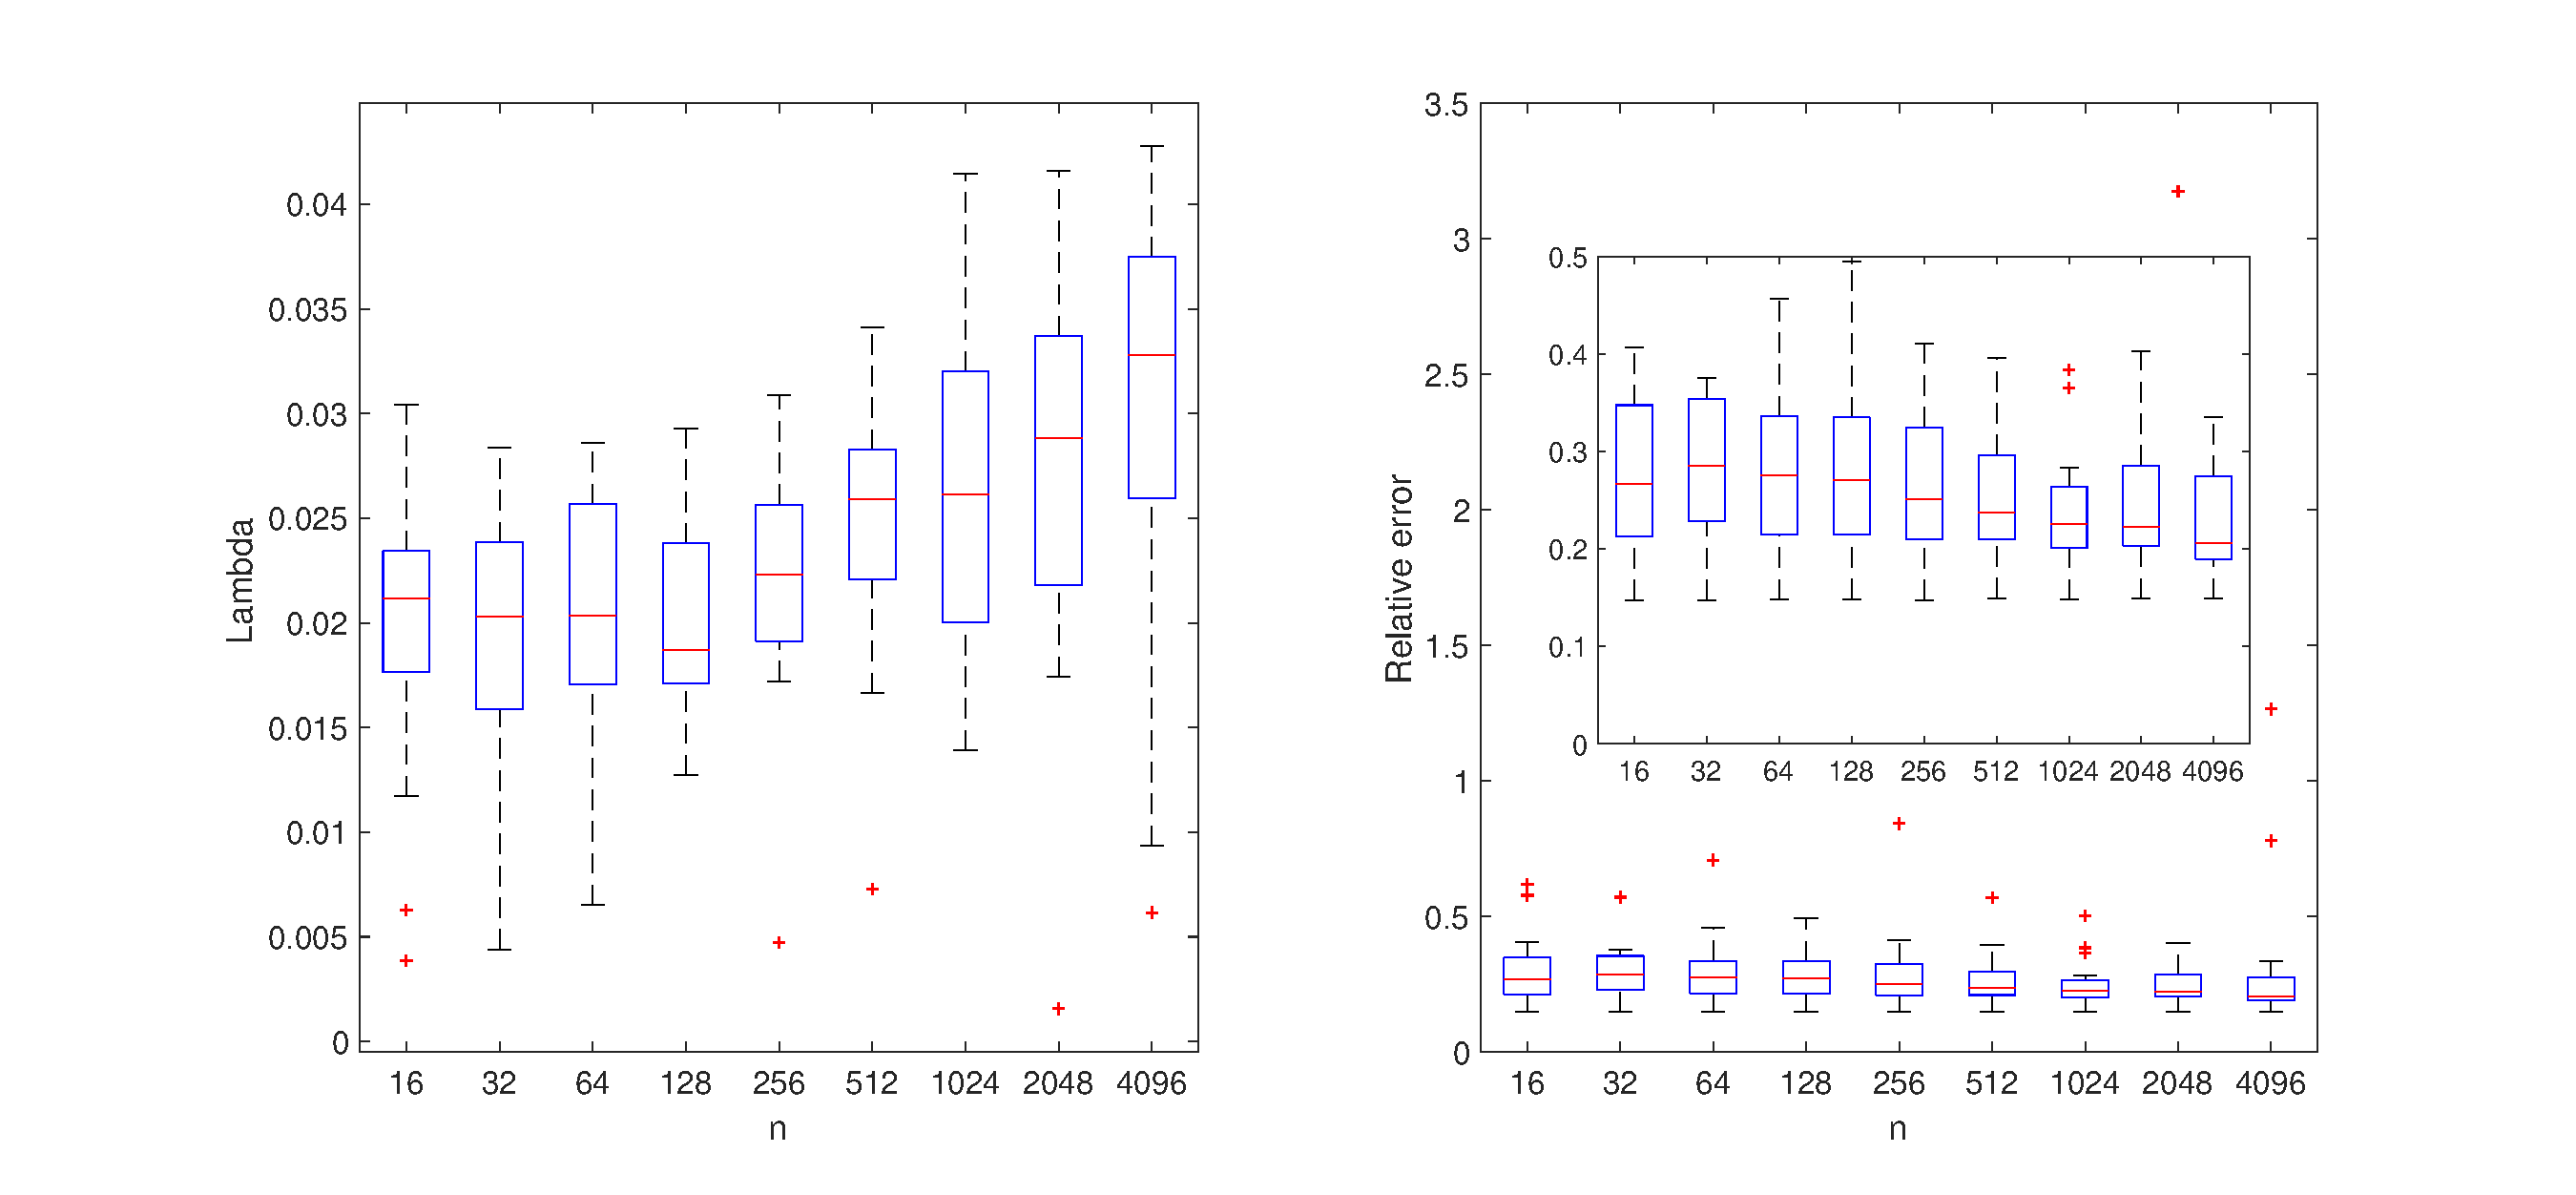
\includegraphics[scale = 0.45]{Figures/BothBoxes1D_F2_S05_W100_R20.eps}}
\caption{Box plots for the regularization parameters $\regparam$ (left) and relative errors (right) across resolutions for 20 noise realizations. In this configuration, $\text{SNR = 5}$ and the width of the Gaussian kernel is 50.}
\end{figure}

\begin{figure}
	\centerline{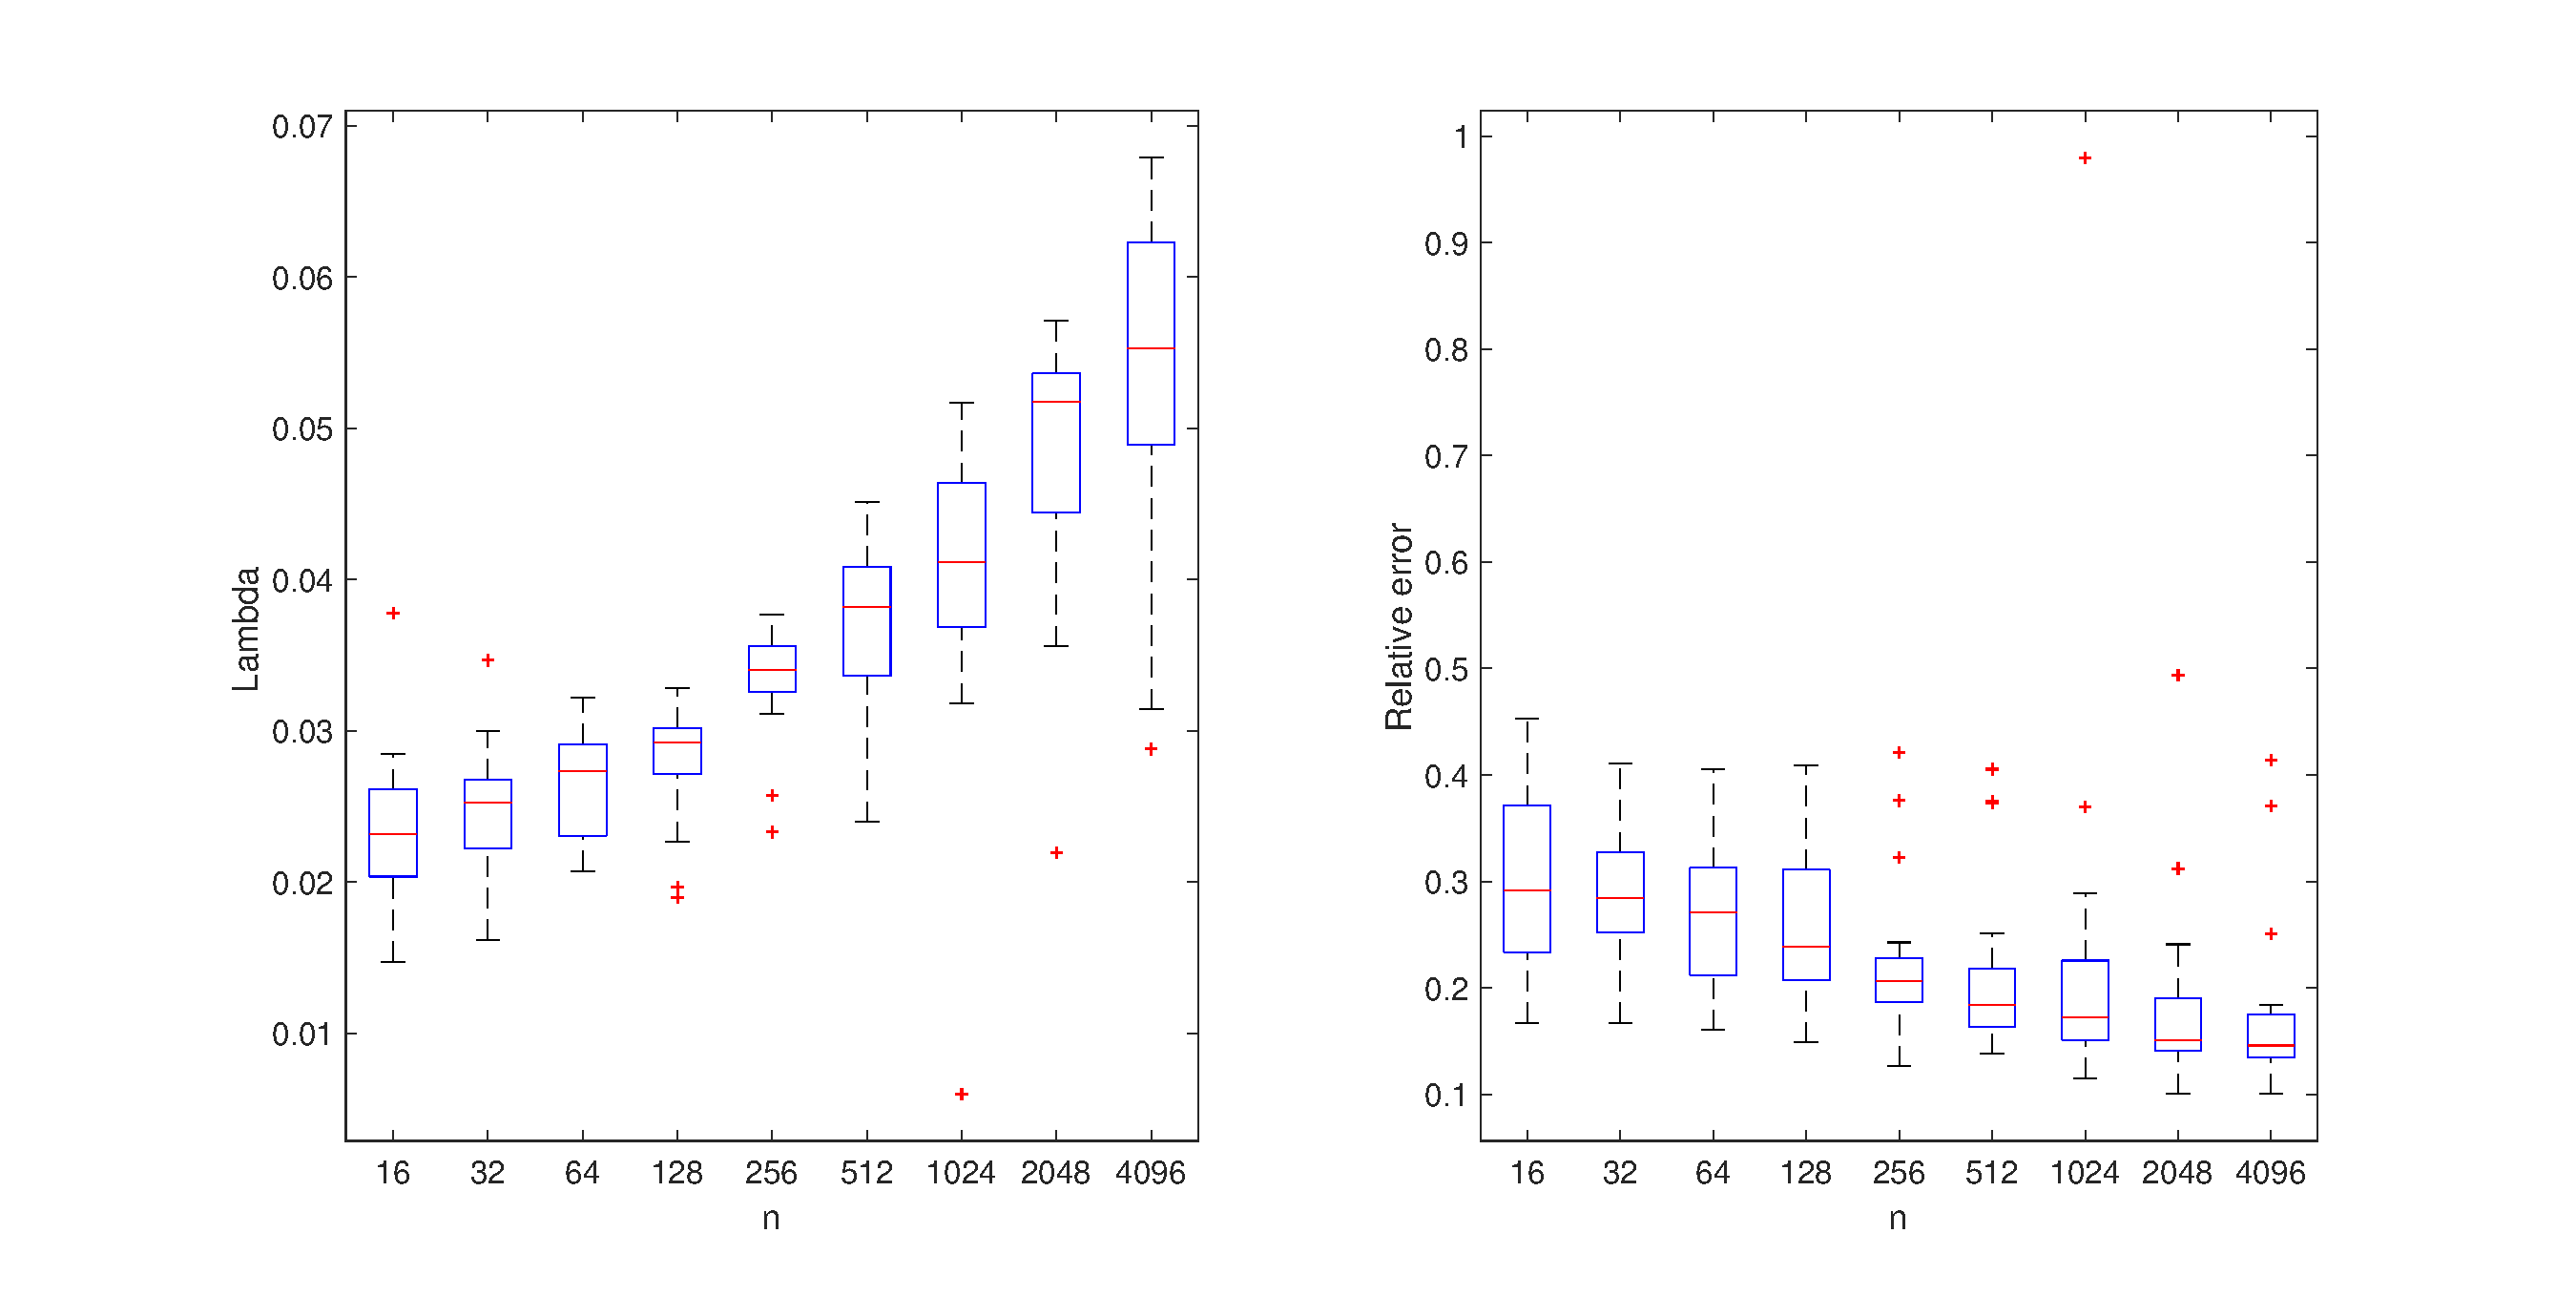
\includegraphics[scale = 0.45]{Figures/BothBoxes1D_F2_S05_W200_R20.eps}}
\caption{Box plots for the regularization parameters $\regparam$ (left) and relative errors (right) across resolutions for 20 noise realizations. In this configuration, $\text{SNR = 25}$ and the width of the Gaussian kernel is 50.}
\end{figure}

\begin{figure}
	\centerline{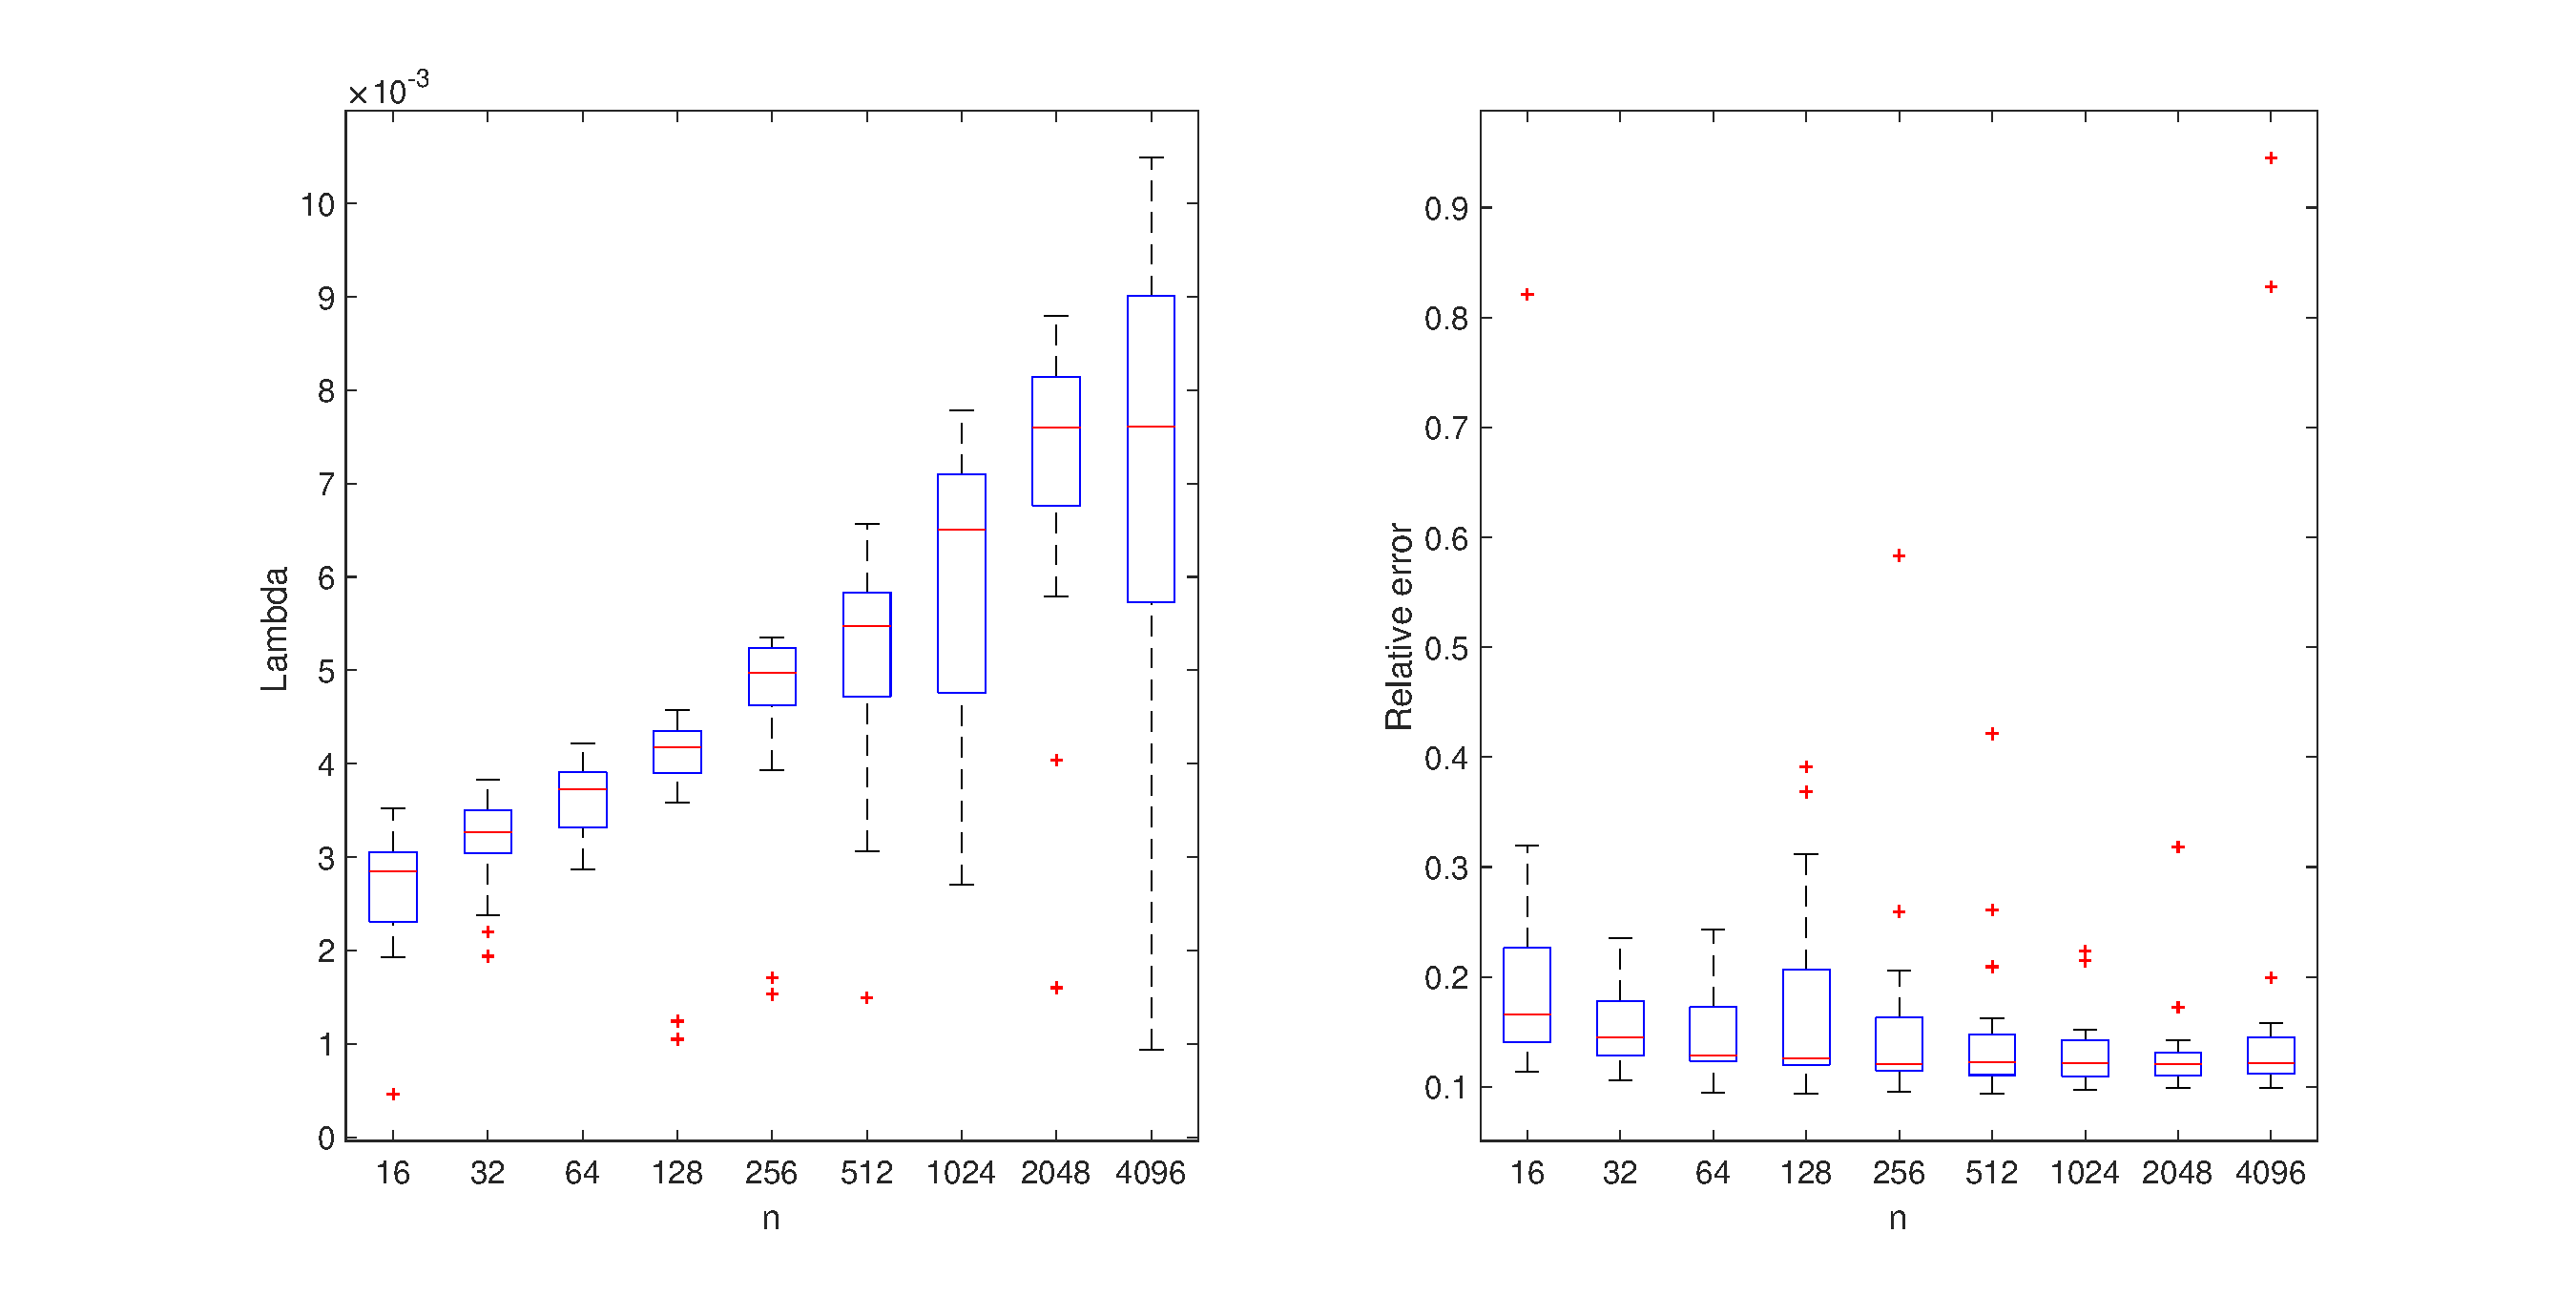
\includegraphics[scale = 0.45]{Figures/BothBoxes1D_F2_S25_W100_R20.eps}}
\caption{Box plots for the regularization parameters $\regparam$ (left) and relative errors (right) across resolutions for 20 noise realizations. In this configuration, $\text{SNR = 5}$ and the width of the Gaussian kernel is 100.}
\end{figure}

\begin{figure}
	\centerline{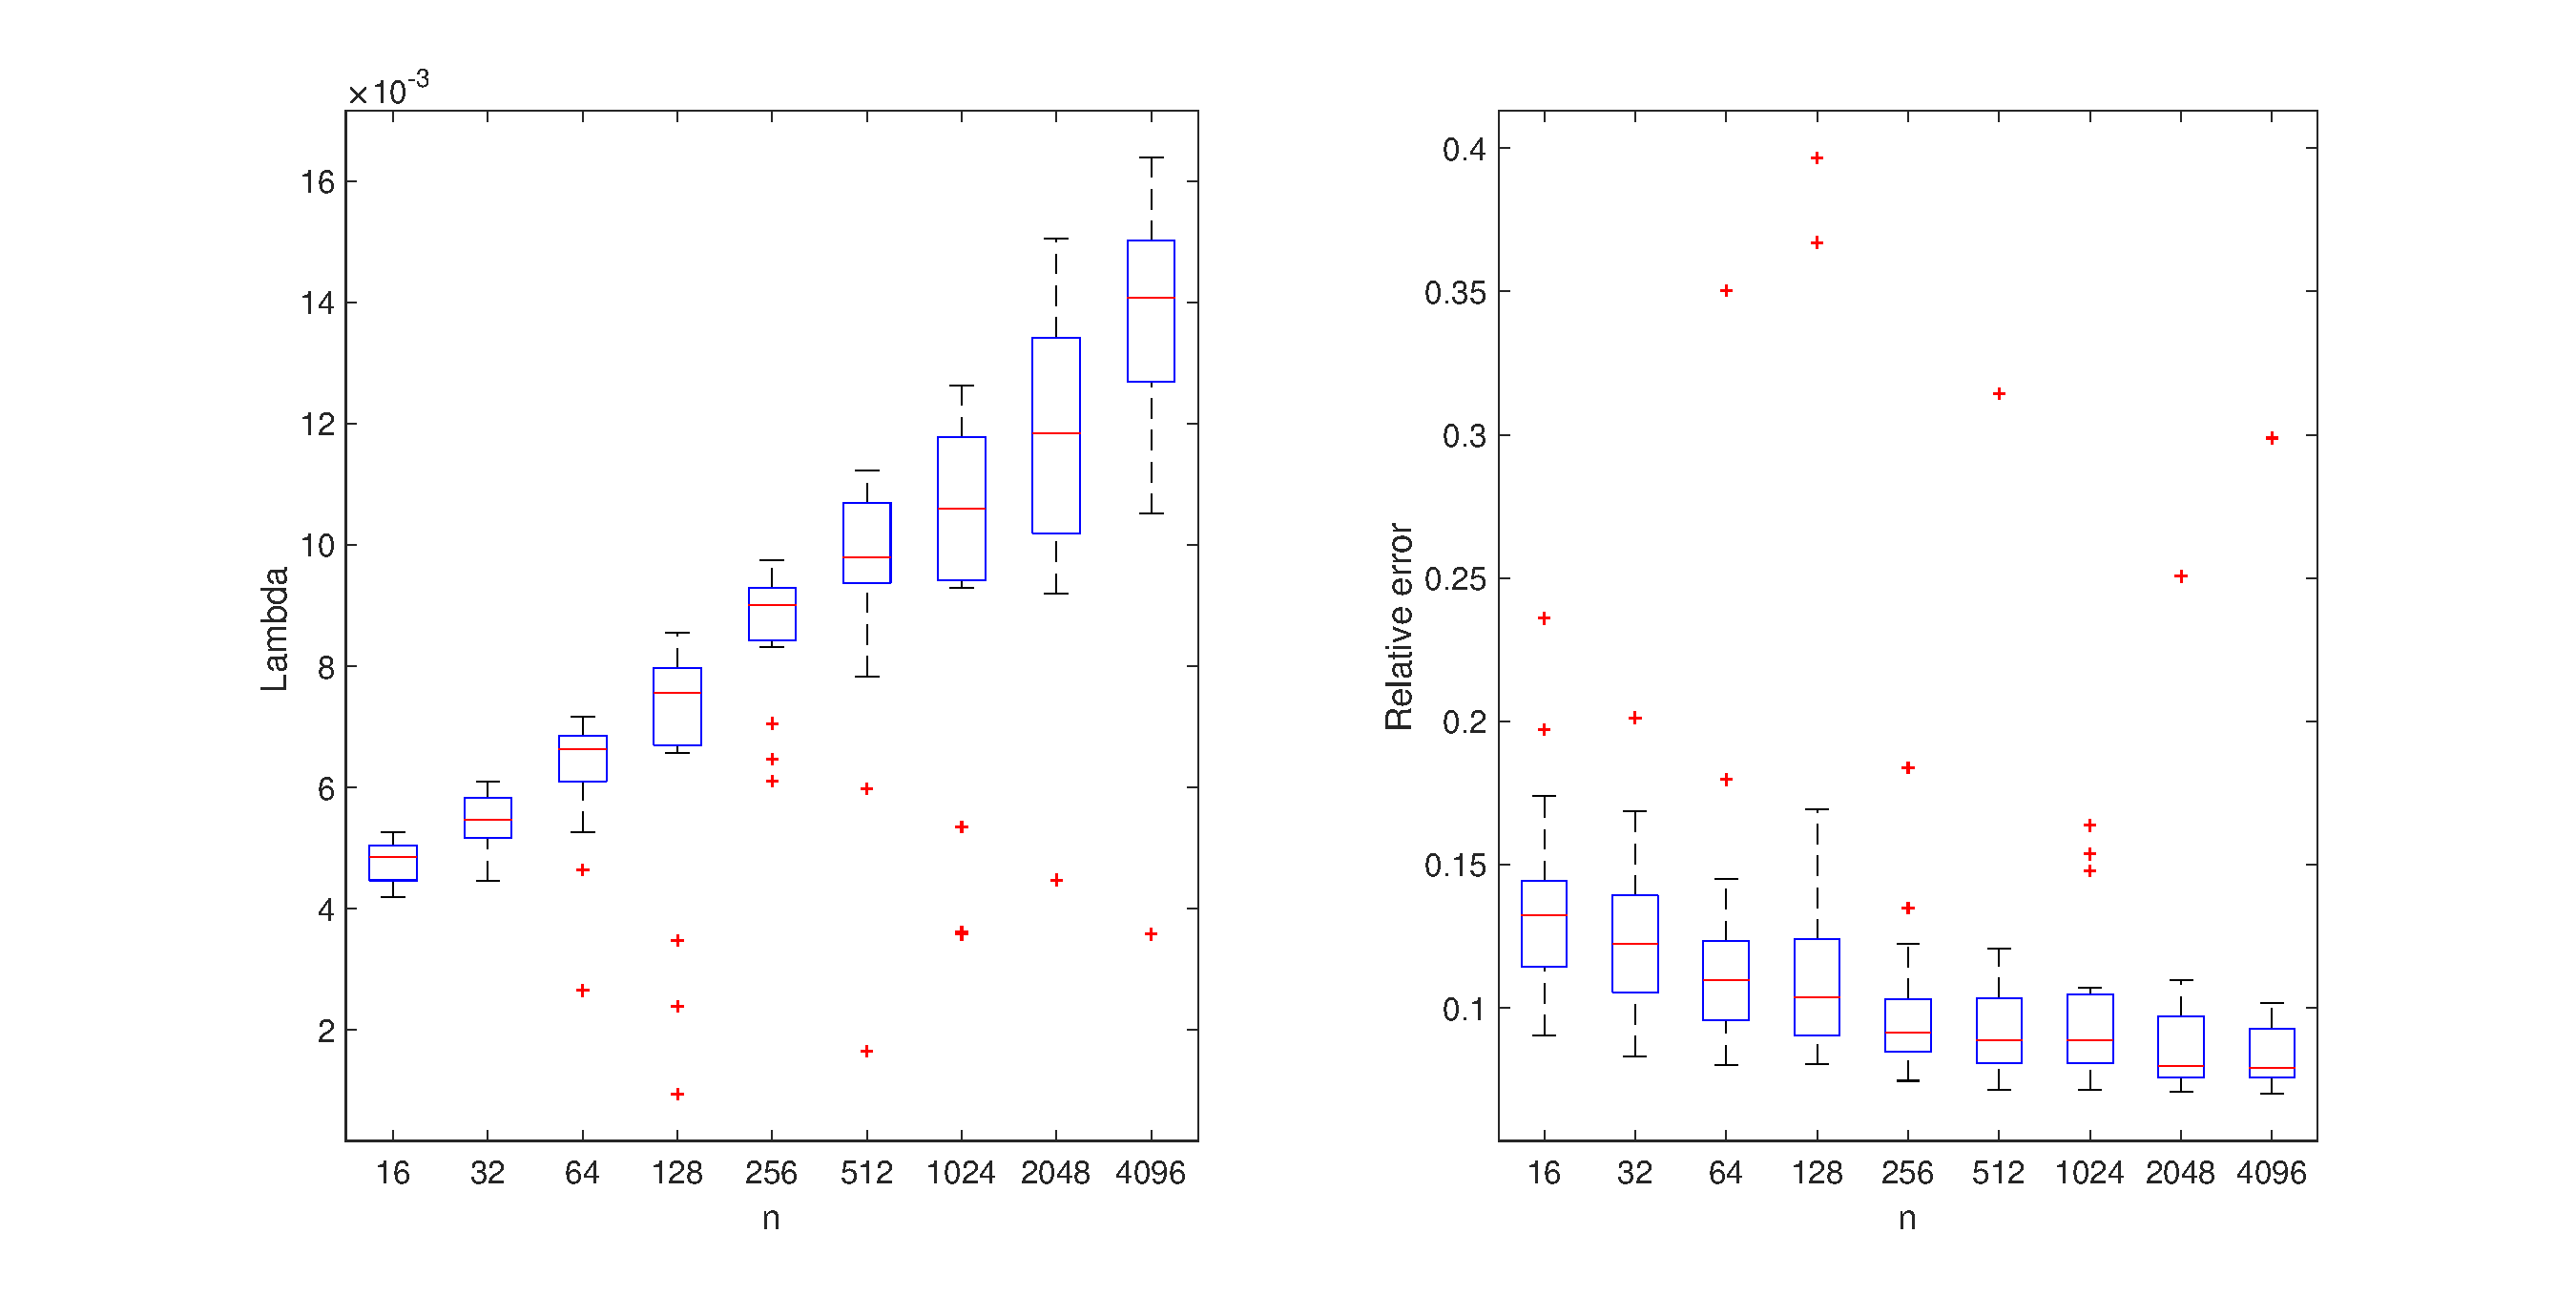
\includegraphics[scale = 0.45]{Figures/BothBoxes1D_F2_S25_W200_R20.eps}}
\caption{Box plots for the regularization parameters $\regparam$ (left) and relative errors (right) across resolutions for 20 noise realizations. In this configuration, $\text{SNR = 25}$ and the width of the Gaussian kernel is 100.}
\end{figure}

It is interesting to note more pronounced increase in the regularization parameter across resolutions when the Gaussian kernel has a width of 100 as opposed to a width of 50. In addition, the relative errors are smaller for an SNR of 25 as opposed to an SNR of 5, which is to be expected since the variance in the noise is small for $\text{SNR} = 25$. 


\section*{References}
\begin{itemize}
	\item[1] Boggess, A., \& Narcowich, F. J. (2009). \textit{A first course in wavelets with Fourier analysis} (2nd ed.). Hoboken, NJ: John Wiley \& Sons.
	\item[2] Debnath, L., \& Mikusi\'{n}ski, P. (2005). \textit{Introduction to Hilbert spaces with applications} (3rd ed.). Elsevier Academic Press.
	\item[3] Vogel, C. R. (2002). \textit{Computational methods for inverse problems} (Frontiers in applied mathematics). Philadelphia, PA: SIAM.
	\item[4] Golub
\end{itemize}


\end{document}